\documentclass[]{tufte-book}

% ams
\usepackage{amssymb,amsmath}

\usepackage{ifxetex,ifluatex}
\usepackage{fixltx2e} % provides \textsubscript
\ifnum 0\ifxetex 1\fi\ifluatex 1\fi=0 % if pdftex
  \usepackage[T1]{fontenc}
  \usepackage[utf8]{inputenc}
\else % if luatex or xelatex
  \makeatletter
  \@ifpackageloaded{fontspec}{}{\usepackage{fontspec}}
  \makeatother
  \defaultfontfeatures{Ligatures=TeX,Scale=MatchLowercase}
  \makeatletter
  \@ifpackageloaded{soul}{
     \renewcommand\allcapsspacing[1]{{\addfontfeature{LetterSpace=15}#1}}
     \renewcommand\smallcapsspacing[1]{{\addfontfeature{LetterSpace=10}#1}}
   }{}
  \makeatother
\fi

% graphix
\usepackage{graphicx}
\setkeys{Gin}{width=\linewidth,totalheight=\textheight,keepaspectratio}

% booktabs
\usepackage{booktabs}

% url
\usepackage{url}

% hyperref
\usepackage{hyperref}

% units.
\usepackage{units}


\setcounter{secnumdepth}{2}

% citations
\usepackage{natbib}
\bibliographystyle{apalike}
%\renewcommand{\bibsection}{\chapter*{References}}

% pandoc syntax highlighting
\usepackage{color}
\usepackage{fancyvrb}
\newcommand{\VerbBar}{|}
\newcommand{\VERB}{\Verb[commandchars=\\\{\}]}
\DefineVerbatimEnvironment{Highlighting}{Verbatim}{commandchars=\\\{\}}
% Add ',fontsize=\small' for more characters per line
\usepackage{framed}
\definecolor{shadecolor}{RGB}{248,248,248}
\newenvironment{Shaded}{\begin{snugshade}}{\end{snugshade}}
\newcommand{\KeywordTok}[1]{\textcolor[rgb]{0.13,0.29,0.53}{\textbf{{#1}}}}
\newcommand{\DataTypeTok}[1]{\textcolor[rgb]{0.13,0.29,0.53}{{#1}}}
\newcommand{\DecValTok}[1]{\textcolor[rgb]{0.00,0.00,0.81}{{#1}}}
\newcommand{\BaseNTok}[1]{\textcolor[rgb]{0.00,0.00,0.81}{{#1}}}
\newcommand{\FloatTok}[1]{\textcolor[rgb]{0.00,0.00,0.81}{{#1}}}
\newcommand{\ConstantTok}[1]{\textcolor[rgb]{0.00,0.00,0.00}{{#1}}}
\newcommand{\CharTok}[1]{\textcolor[rgb]{0.31,0.60,0.02}{{#1}}}
\newcommand{\SpecialCharTok}[1]{\textcolor[rgb]{0.00,0.00,0.00}{{#1}}}
\newcommand{\StringTok}[1]{\textcolor[rgb]{0.31,0.60,0.02}{{#1}}}
\newcommand{\VerbatimStringTok}[1]{\textcolor[rgb]{0.31,0.60,0.02}{{#1}}}
\newcommand{\SpecialStringTok}[1]{\textcolor[rgb]{0.31,0.60,0.02}{{#1}}}
\newcommand{\ImportTok}[1]{{#1}}
\newcommand{\CommentTok}[1]{\textcolor[rgb]{0.56,0.35,0.01}{\textit{{#1}}}}
\newcommand{\DocumentationTok}[1]{\textcolor[rgb]{0.56,0.35,0.01}{\textbf{\textit{{#1}}}}}
\newcommand{\AnnotationTok}[1]{\textcolor[rgb]{0.56,0.35,0.01}{\textbf{\textit{{#1}}}}}
\newcommand{\CommentVarTok}[1]{\textcolor[rgb]{0.56,0.35,0.01}{\textbf{\textit{{#1}}}}}
\newcommand{\OtherTok}[1]{\textcolor[rgb]{0.56,0.35,0.01}{{#1}}}
\newcommand{\FunctionTok}[1]{\textcolor[rgb]{0.00,0.00,0.00}{{#1}}}
\newcommand{\VariableTok}[1]{\textcolor[rgb]{0.00,0.00,0.00}{{#1}}}
\newcommand{\ControlFlowTok}[1]{\textcolor[rgb]{0.13,0.29,0.53}{\textbf{{#1}}}}
\newcommand{\OperatorTok}[1]{\textcolor[rgb]{0.81,0.36,0.00}{\textbf{{#1}}}}
\newcommand{\BuiltInTok}[1]{{#1}}
\newcommand{\ExtensionTok}[1]{{#1}}
\newcommand{\PreprocessorTok}[1]{\textcolor[rgb]{0.56,0.35,0.01}{\textit{{#1}}}}
\newcommand{\AttributeTok}[1]{\textcolor[rgb]{0.77,0.63,0.00}{{#1}}}
\newcommand{\RegionMarkerTok}[1]{{#1}}
\newcommand{\InformationTok}[1]{\textcolor[rgb]{0.56,0.35,0.01}{\textbf{\textit{{#1}}}}}
\newcommand{\WarningTok}[1]{\textcolor[rgb]{0.56,0.35,0.01}{\textbf{\textit{{#1}}}}}
\newcommand{\AlertTok}[1]{\textcolor[rgb]{0.94,0.16,0.16}{{#1}}}
\newcommand{\ErrorTok}[1]{\textcolor[rgb]{0.64,0.00,0.00}{\textbf{{#1}}}}
\newcommand{\NormalTok}[1]{{#1}}

% longtable
\usepackage{longtable,booktabs}

% multiplecol
\usepackage{multicol}

% strikeout
\usepackage[normalem]{ulem}

% morefloats
\usepackage{morefloats}

% force floats added by CII
\usepackage{float}
\floatplacement{figure}{H}


% tightlist macro required by pandoc >= 1.14
\providecommand{\tightlist}{%
  \setlength{\itemsep}{0pt}\setlength{\parskip}{0pt}}

% title / author / date
\title{Getting used to R, RStudio, and R Markdown}

\author{Chester Ismay}
\date{2017-03-20}

\usepackage{booktabs}
\usepackage{longtable}
\usepackage{framed,color}
\usepackage{float}
\floatplacement{figure}{H}
\usepackage[parfill]{parskip}
\definecolor{shadecolor}{RGB}{248,248,248}

\ifxetex
  \usepackage{letltxmacro}
  \setlength{\XeTeXLinkMargin}{1pt}
  \LetLtxMacro\SavedIncludeGraphics\includegraphics
  \def\includegraphics#1#{% #1 catches optional stuff (star/opt. arg.)
    \IncludeGraphicsAux{#1}%
  }%
  \newcommand*{\IncludeGraphicsAux}[2]{%
    \XeTeXLinkBox{%
      \SavedIncludeGraphics#1{#2}%
    }%
  }%
\fi

%% Need to clean up
\newenvironment{rmdblock}[1]
  {\begin{shaded*}
  \begin{itemize}
  \renewcommand{\labelitemi}{
    \raisebox{-.7\height}[0pt][0pt]{
  %    {\setkeys{Gin}{width=3em,keepaspectratio}\includegraphics{images/#1}}
    }
  }
  \item
  }
  {
  \end{itemize}
  \end{shaded*}
  }
%% Probably can be omitted
\newenvironment{rmdnote}
  {\begin{rmdblock}{note}}
  {\end{rmdblock}}
\newenvironment{rmdcaution}
  {\begin{rmdblock}{caution}}
  {\end{rmdblock}}
\newenvironment{rmdimportant}
  {\begin{rmdblock}{important}}
  {\end{rmdblock}}
\newenvironment{rmdtip}
  {\begin{rmdblock}{tip}}
  {\end{rmdblock}}
\newenvironment{rmdwarning}
  {\begin{rmdblock}{warning}}
  {\end{rmdblock}}
\newenvironment{learncheck}
  {\begin{rmdblock}{warning}}
  {\end{rmdblock}}
\newenvironment{review}
  {\begin{rmdblock}{warning}}
  {\end{rmdblock}}

% To tweak tufte layout
\geometry{
  left=0.8in, % left margin
  textwidth=35pc, % main text block
  marginparsep=1pc, % gutter between main text block and margin notes
  marginparwidth=8pc % width of margin notes
}

\usepackage{amsthm}
\newtheorem{theorem}{Theorem}[chapter]
\newtheorem{lemma}{Lemma}[chapter]
\theoremstyle{definition}
\newtheorem{definition}{Definition}[chapter]
\newtheorem{corollary}{Corollary}[chapter]
\newtheorem{proposition}{Proposition}[chapter]
\theoremstyle{definition}
\newtheorem{example}{Example}[chapter]
\theoremstyle{remark}
\newtheorem*{remark}{Remark}
\begin{document}

%\let\allcaps=\relax
\maketitle



{
\setcounter{tocdepth}{1}
\tableofcontents
}

\chapter{Introduction}\label{intro}

In the HTML version of this book, you can also download the PDF version
of the book by clicking on PDF button in the top toolbar of the page.
HTML is the preferred format but the PDF format may be preferred for
some readers. Links to the different GIFs directly found in the HTML
version are provided in the PDF version.

This resource is designed to provide new users to R, RStudio, and R
Markdown with the introductory steps needed to begin their own
reproducible research. Many screenshots and GIFs will be included, but
if further clarification is needed on these or any other aspect of the
book, please create a GitHub issue
\href{https://github.com/ismayc/rbasics-book/issues}{here} or email
\href{mailto:chester.ismay@gmail.com}{me} with a reference to the
error/area where more guidance is necessary. Pull requests on GitHub for
typos or improvements are preferred and you can easily do so by clicking
on the Edit button near Search at the top of the HTML version of the
book.

This book will evolve and be updated as needed based on feedback. You
can always check the date below to see when the book was last updated.

It is recommended that you have R version 3.3.0 or later, RStudio
Desktop version 0.99 or higher, and \texttt{rmarkdown} R package version
1.0 or higher. This is to make sure that the screenshots and GIF
recordings match up with the behavior on your machine/set-up.
Additionally, you may find that GIFs don't load sometimes. I haven't had
any problems using Google Chrome and recommend that as your browser to
view this book if you have troubles with others.

This book was last updated by cismay on Monday, March 20, 2017 11:35:51
PDT.

\chapter{Why R?}\label{whyR}

If you are brand new to R and programming, you may be scared. You aren't
used to having to type commands to tell the computer what to do. You may
be more used to using drop-down menus and other graphical user
interfaces that allow you to pick what you'd like to do. So why are so
many companies, colleges/universities, and individuals of all
disciplinary backgrounds shifting towards using R?

There are lots of answers to this question, but some of the most
important for us now are:

\begin{enumerate}
\def\labelenumi{\arabic{enumi}.}
\item
  R is free. RStudio is free.

  One of the biggest perks about working with R and RStudio is that they
  are both provided free of charge to use. R is an open-source
  programming language that has grown tremendously in recent years with
  developers adding more functionality and packages on a daily basis.
  Where other more proprietary packages are sometimes stuck in the dark
  ages (the 1990s, for example) of development and can be incredibly
  expensive to purchase, R continues to be a free alternative that
  allows users of all levels to contribute.

  RStudio is a graphical user interface that allows one to write R code
  and view the results of that code in an easy way. It is also free to
  download and work with.
\item
  Analyses done using R are reproducible.

  As many scientific fields push towards more reproducible analyses, the
  point-and-click proprietary systems actually serve as a hindrance to
  this process. If you need to re-run your analysis using these systems,
  you'll need to carefully copy-and-paste your analysis and plots into
  your text editors from potentially beginning to end. Anyone that has
  done this sort of copy-and-pasting knows that it is prone to errors
  and incredibly tedious.

  If you use the workflows described in this book, your analyses will be
  reproducible so you don't need to worry about these copy-and-pasting
  issues. As you might have guessed by now, it would be much better to
  be able to update your code/data inputs and re-run all of your
  analysis than to have to worry about manually moving your results from
  one program to another. Reproducibility also helps you as a programmer
  since your greatest collaborator will probably be yourself a few
  months or years down the road. Instead of having to carefully write
  down all the steps you took to find the right drop-down menu option,
  your entire code is stored.
\item
  Using R makes collaboration easier.

  This also helps you with collaboration since, as you will see later,
  you can share an R Markdown file containing all of your analysis,
  documentation, commentary, and the code to others. This reduces the
  time to needed to work with others and reduces the likelihood of
  errors being made in following along with point-and-click analyses.
  The mantra here will be to \textbf{Say No to Copy-And-Paste!} both for
  your sanity and for the sake of science.
\item
  Finding answers to questions is much simpler.

  If you have ever had an issue with software, you know how difficult it
  is to find answers to your questions. ``How can I describe the process
  to someone else? Do I need to take screenshots? Do I really need to
  call IT and wait for hours for someone to respond?'' R is a
  programming language and so it is much easier (after a bit of
  practice) to use Google or Stack Overflow to find answers to your
  questions. You'll be amazed at how many other users have encountered
  the same sorts of errors you will see when you begin.

  I frequently (almost on a daily basis) Google things like ``How do I
  make a side-by-side boxplot in R coloring by a third variable?''.
  You'll become better at working with R by reaching out to others for
  help and by answering questions that others have. In addition, Chapter
  \ref{errors} describes many common errors and how you can fix them.
\item
  Struggling through programming helps you learn.

  We all know that learning isn't easy. Do you have trouble remembering
  how to follow a list of more than 10 steps or so? Do you find yourself
  going back over and over again because you can't remember what step
  comes next in the process? This is extremely common especially if you
  haven't done the procedure in awhile. Learning via following a
  procedure is easy in the short-term, but can be extremely frustrating
  to remember in the long-term. Programming (if done well) promotes
  long-term thinking to short-term fixes.

  One unfortunate thing that we frequently take for granted is that our
  brain tricks us into picking the easy route. If you truly want to
  learn how to do something (like programming with R), you'll need to
  feel frustrated at times. Any time you learn something you've been
  frustrated. (We tend to forget all the frustration and only think
  about where we currently are.) R still frustrates me from time to
  time, but I grow through practice and I look forward to the
  challenges. Hadley Wickham encapsulated this phenomenon nicely in the
  Prologue of the book ``Hands-On Programming with R''
  \citep{handson2014}:

  \begin{quote}
  As you learn to program, you are going to get frustrated. You are
  learning a new language, and it will take time to become fluent. But
  frustration is not just natural, it's actually a positive sign that
  you should watch for. Frustration is your brain's way of being lazy;
  it's trying to get you to quit and go do something easy or fun. If you
  want to get physically fitter, you need to push your body even though
  it complains. If you want to get better at programming, you'll need to
  push your brain. Recognize when you get frustrated and see it as a
  good thing: you're now stretching yourself. Push yourself a little
  further every day, and you'll soon be a confident programmer.
  \end{quote}
\end{enumerate}

\chapter{R and RStudio Basics}\label{rstudiobasics}

\section{What is R?}\label{what-is-r}

In Chapter \ref{whyR}, I discussed many of the reasons why you should be
doing your analyses (especially those of the data type) using R. If you
skipped over that chapter in the hopes of just hopping into learning
about R, I request that you to go back to it and carefully read it over.
As you begin working with R, it is especially important to review that
introductory chapter from time to time.

\subsection{R beginnings}\label{r-beginnings}

R was created by a group of statisticians who wanted an open-source
alternative to the costly proprietary options. Being created by
statisticians (instead of computer scientists) means that R has some
quirky aspects to it that take a little bit of time to get used to.
We'll see that many packages have been developed to help with this and
that you don't need to have advanced degrees in Statistics to be able to
work with R now.

Getting back to the development of R\ldots{} R was created by
\textbf{R}oss Ihaka and \textbf{R}obert Gentleman in New Zealand at the
University of Auckland. It is a spin-off of the S programming language
and is named partly after the first names of its developers (as you can
see in the emphasis above). The beginning ideas for creating R came in
1992 and the first version of R was released in 1994. You can find much
more about the background of R and its features as well as its
connections to the S language on its
\href{https://en.wikipedia.org/wiki/R_(programming_language)}{Wikipedia
page}.

\subsection{R packages}\label{r-packages}

I first learned to use R while a graduate student at Northern Arizona
University from \href{http://www.stat.colostate.edu/~pturk/}{Dr.~Philip
Turk} in 2007. At the time, I never thought that R could have exploded
in users as we have seen since 2011. I never would have thought that
students taking an introductory statistics course would be encouraged to
learn to use R.

In 2007, it was still largely esoteric and tricky language used by
statisticians to do analyses. Getting used to the syntax for producing
plots and working with data was especially tricky for those with little
to no programming experience. So what has changed since 2007 about
learning R?

I believe one of the biggest developments has been the creation of
packages to make R easier to work with for newbies. Packages are created
by users of R to increase the functionality of the base R installation.
Packages created by Hadley Wickham and others recently have greatly
expanded the capabilities of R, while also working to make beginning
with R simpler. From the Wikipedia page referenced earlier, as of
January 2016, there were around 7800 additional R packages available on
common R repositories.\footnote{You'll see how to download these
  packages via \texttt{install.packages("dplyr")} and load them into
  your current R working environment via \texttt{library("dplyr")}, for
  example, in Chapter \ref{rmdanal}.}

Another great development is the graphical user interface called RStudio
and the package developed by the those that work for RStudio, Inc.
called \texttt{rmarkdown}. We will discuss \texttt{rmarkdown} (also
referred to as R Markdown) in a Chapter \ref{rmarkdown}, and will now
focus on discussing RStudio.

\section{What is RStudio?}\label{what-is-rstudio}

RStudio is a powerful, free, open-source integrated development
environment for R. It began development in 2010 and its first beta
release came in February 2011. It is available in two editions: RStudio
Desktop and RStudio Server. This book will focus mostly on using the
RStudio Server, but both versions are nearly identical to work with.

You can find instructions linked below for downloading R and RStudio on
Windows and Mac machines. If you are using RStudio Server, your
professor and members of your organization's IT department have done
these steps for you. On the RStudio Server you log on using a web
browser to an account sitting on the cloud. There are many advantages to
using the RStudio Server for the beginning user including sharing of R
projects to help with feedback and error resolution. Installation of
software can also cause its own headaches and this is eliminated by
using the RStudio Server.

\textbf{Note for advanced users}: You can also install your very own
RStudio Server for around \$5 per month on Digital Ocean. Instructions
to do so can be found from Dean Attali
\href{http://deanattali.com/2015/05/09/setup-rstudio-shiny-server-digital-ocean/}{here}
and on the Digital Ocean site
\href{https://www.digitalocean.com/community/tutorials/how-to-set-up-rstudio-on-an-ubuntu-cloud-server}{here}.

After you complete a few months of work with the RStudio Server, it is
recommended that you download RStudio Desktop to your computer. The
instructions to do so are below.

\subsection{Installing R and RStudio
Desktop}\label{installing-r-and-rstudio-desktop}

It is worth noting that you can't just install RStudio Desktop without
installing R as RStudio needs to have R installed in order to run. A
step-by-step guide to installing R and RStudio Desktop with screenshots
can be found

\begin{itemize}
\tightlist
\item
  \href{http://www.reed.edu/data-at-reed/software/R/r_studio.html}{here}
  for the Mac and
\item
  \href{http://www.reed.edu/data-at-reed/software/R/r_studio_pc.html}{here}
  for a PC.
\end{itemize}

Unless you plan to create PDF documents (which requires a multiple
gigabyte download of LaTeX) you can skip some of the later steps of the
installation. It is recommended that you select \textbf{HTML} as the
Default Output Format for R Markdown. You'll see more about this in
Chapter \ref{rmarkdown}.

\section{Working in RStudio Server}\label{working-in-rstudio-server}

\subsection{Logging in and initial
screen}\label{logging-in-and-initial-screen}

The RStudio Server provides a web-based way to run analyses in R. This
means that you will only need an internet connection and a web browser
to run your analyses. Your professor or administrator will provide you
with a link to the web location of your RStudio Server. After entering
the link, you'll see a page that looks something like:

\begin{figure}

{\centering 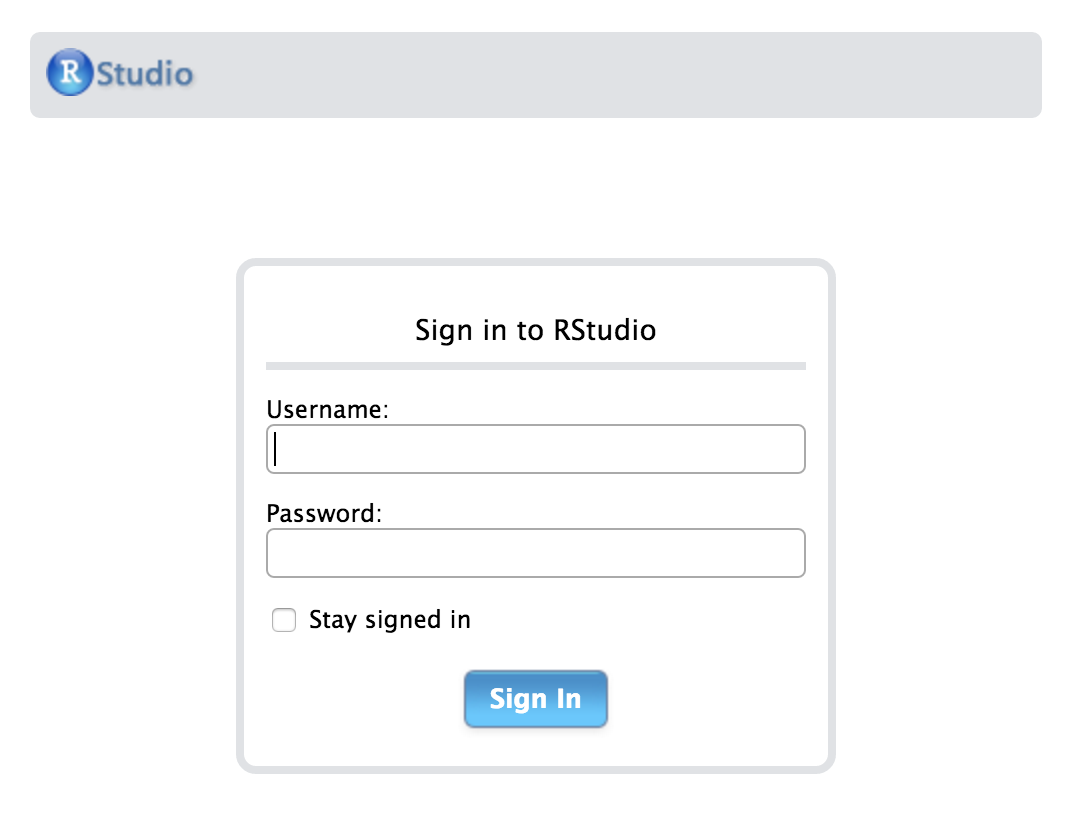
\includegraphics[width=\textwidth]{screenshots/server_login} 

}

\caption[Login page for RStudio Server]{Login page for RStudio Server}\label{fig:serverlogin}
\end{figure}

After logging in with your username and password, you should see a
layout similar to what follows.

\begin{figure}

{\centering 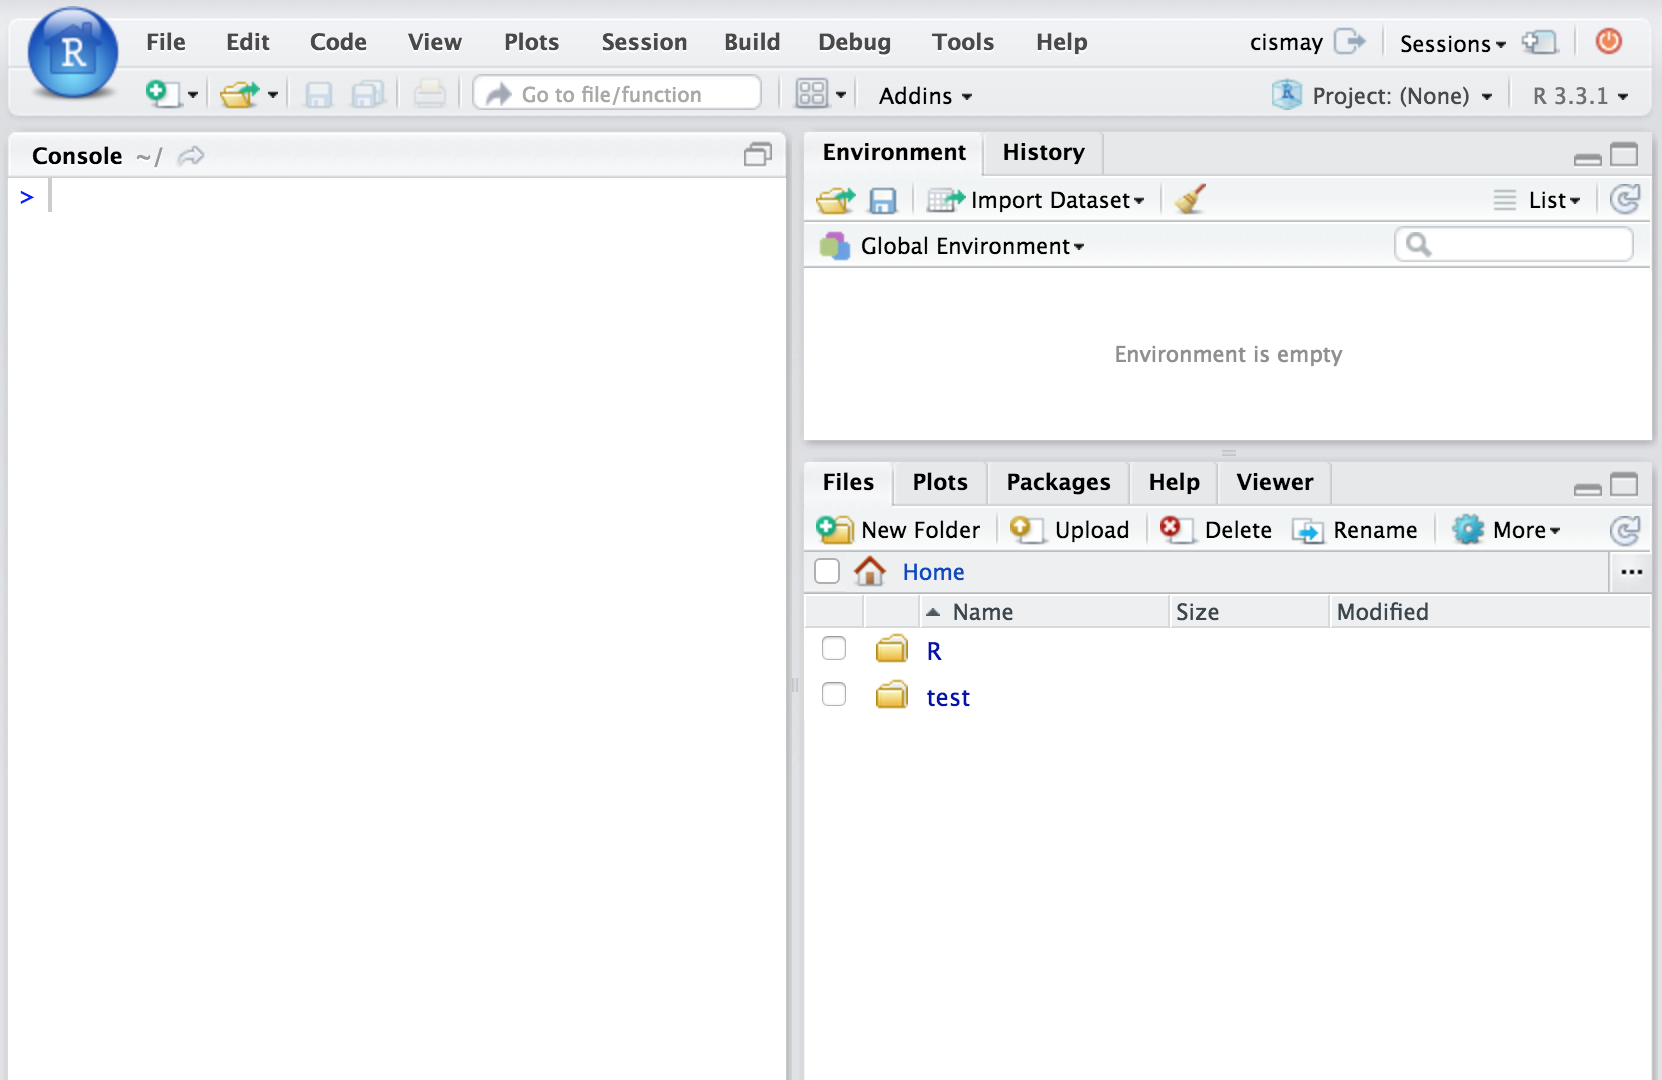
\includegraphics[width=\textwidth]{screenshots/initial_rstudio} 

}

\caption[Initial page for RStudio Server]{Initial page for RStudio Server}\label{fig:initialrstudio}
\end{figure}

For your own reference, a screenshot of RStudio Desktop looks like:

\begin{figure}

{\centering 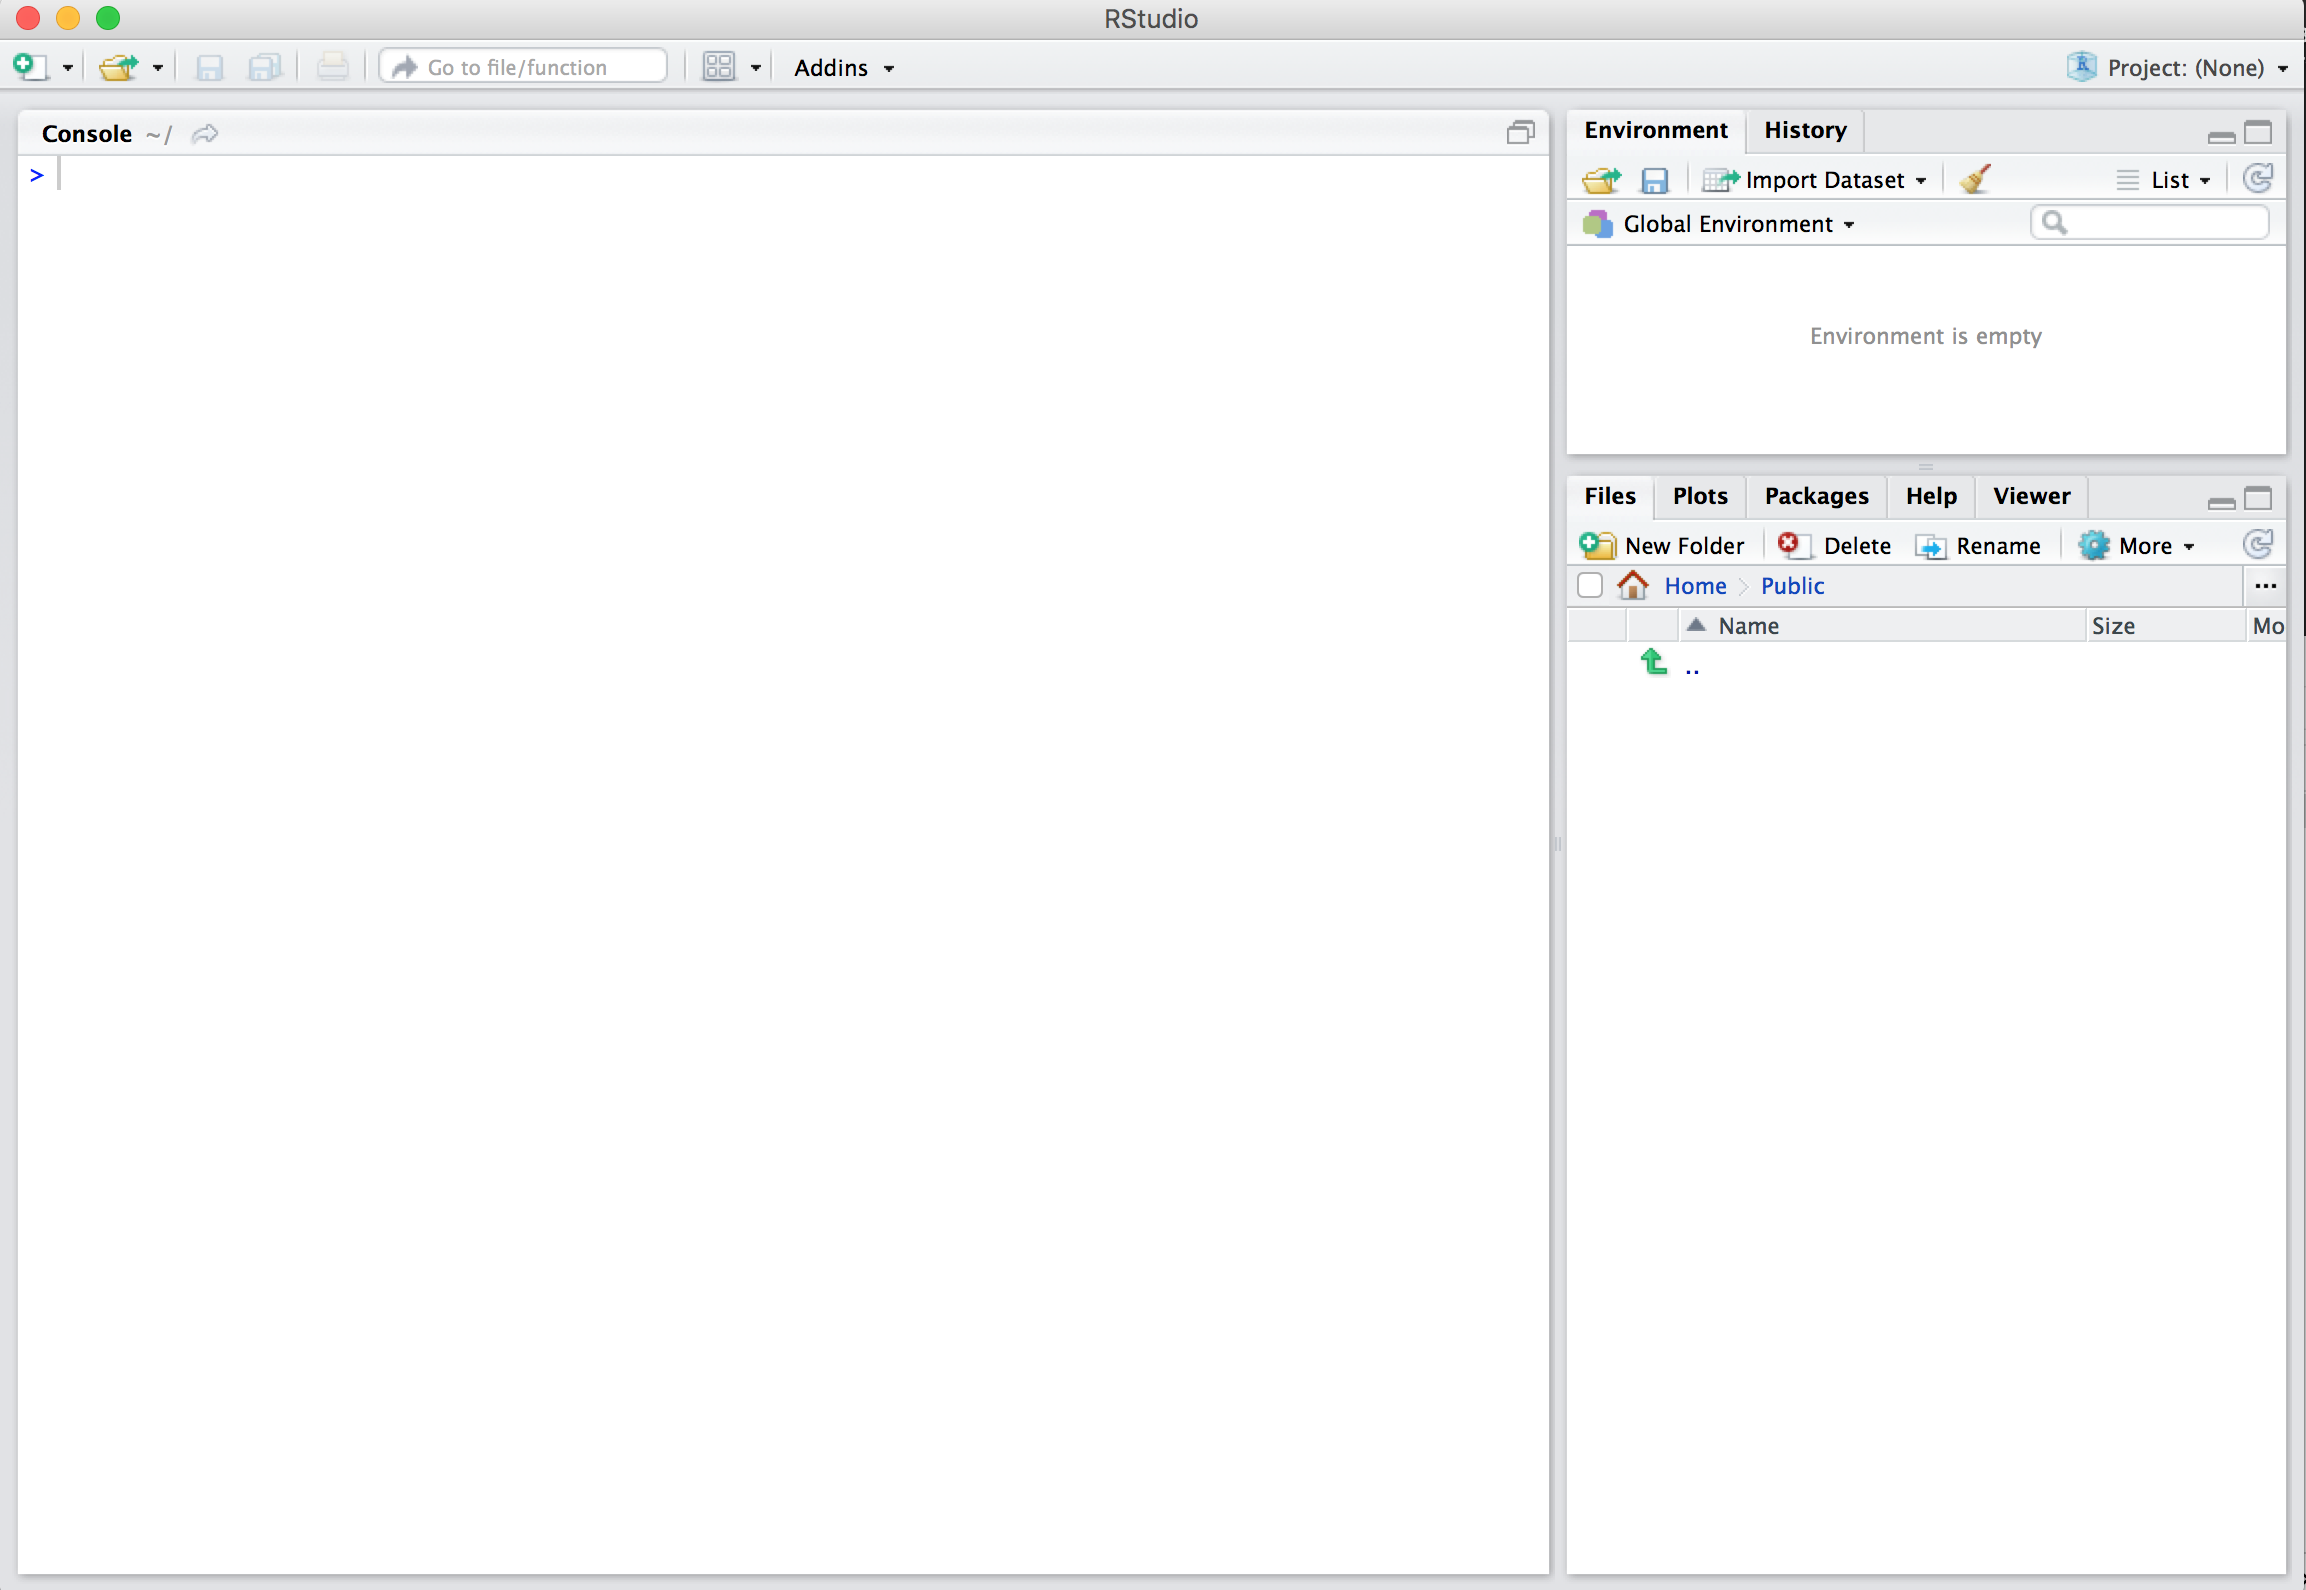
\includegraphics[width=\textwidth]{screenshots/desktop_initial} 

}

\caption[Initial page for RStudio Desktop]{Initial page for RStudio Desktop}\label{fig:initialdesktop}
\end{figure}

As you can see they are almost identical. This makes working between the
two different RStudio set-ups painless. A discussion of what each of the
three different RStudio panes (will soon be four panes) and their
corresponding tabs will occur in Chapter \ref{rmarkdown}. You'll find
that a lot of what follows also applies to RStudio Desktop (except for
the Shared Projects feature), but it always recommended to create an
RStudio project regardless of whether you are on the cloud or working
locally.

\subsection{Basic Workflow with
RStudio}\label{basic-workflow-with-rstudio}

A good habit to get into whenever you start a new project with R code is
to create a new RStudio project to go along with it. RStudio project
files have the extension \texttt{.Rproj} and store metadata that goes
along with the documents you've saved and information about the R
environment you are working in. More information about RStudio projects
is available from RStudio, Inc.
\href{https://support.rstudio.com/hc/en-us/articles/200526207-Using-Projects}{here}.

If you are sharing homework or lab assignments with your instructor
using RStudio Server, for example, it might make sense to create an
RStudio project, share it with your instructor, and then create new
folders for each lab. We will follow this example below.

The GIF below shows you how to create a new RStudio project called
\texttt{initial} and also your first R Markdown file. Note that you also
may see a description about what version of R is running on your initial
login like shown in the GIF below in the Console pane.

\vspace{0.1in}

\begin{center}\footnotesize{\url{https://raw.githubusercontent.com/ismayc/rbasics-book/gh-pages/gifs/proj_rmd.gif}}\end{center}

\vspace{0.1in}

We have our \textbf{first\_rmarkdown.Rmd} file set up.

\subsection{Sharing Projects on RStudio Server
Pro}\label{sharing-projects-on-rstudio-server-pro}

You will now see an example of how to share this project with another
user. This will enable you and collaborators (other students, your
instructor, etc.) to work on the \textbf{Rmd} file at the same time.
This is similar to working on a Google Doc at the same time as someone
else.

RStudio Server comes in a couple different formats and you'll need to
make sure you (or your IT administrator) have installed RStudio Server
Pro to use the Shared Projects feature. You can find more information
from RStudio, Inc. on this
\href{https://support.rstudio.com/hc/en-us/articles/211659737-Sharing-Projects-in-RStudio-Server-Pro}{here}.
Below is an example GIF of sharing this \textbf{initial.Rproj} project
file with another user of the RStudio Server.

\vspace{0.1in}

\begin{center}\footnotesize{\url{https://raw.githubusercontent.com/ismayc/rbasics-book/gh-pages/gifs/share_proj.gif}}\end{center}

\vspace{0.1in}

Both myself and \texttt{bottk} can now work together on this project. We
can type our commentary and code into \textbf{first\_rmarkdown.Rmd} or
other files and save files to the common folder where
\textbf{initial.Rproj} resides.

In Chapter \ref{rmarkdown}, you'll see why it is recommended you work in
R Markdown files and you'll also begin to see some examples of how R
works with R Markdown.

\section{RStudio Layout}\label{rstudio-layout}

You may be initially a little overwhelmed by all the different panes and
tabs that are available in RStudio. You'll soon learn to love this
layout but, as with all things, it will take a little bit to get used to
it. We will begin with the top left pane, proceed to the top right pane,
then to the bottom left pane, and lastly to the bottom right pane. These
panes can be customized but it is recommended for beginning users to
keep things in this standard layout.

\subsection{Code Editor / View Window}\label{code-editor-view-window}

Likely the pane where you will spend a majority of your time is in the
top left. When you first login this pane isn't there, but it was created
when we made the \textbf{first\_rmarkdown.Rmd}. This pane serves as a
place to view the contents of files and objects in R. In the GIF below,
you can see that we can change the text in this file and then save the
file.

Note that the tab that gives the filename will change its color from
black to red and an asterisk will appear after the filename. This is to
remind you that the file is not saved. You'll need to get into the habit
of saving files frequently. You can have multiple tabs open and view
different files in this pane. You'll also see that you can \texttt{View}
datasets in this pane in Chapter \ref{rmarkdown}.

\vspace{0.1in}

\begin{center}\footnotesize{\url{https://raw.githubusercontent.com/ismayc/rbasics-book/gh-pages/gifs/top_left_pane.gif}}\end{center}

\vspace{0.1in}

It may not be clear what these additions are really doing just yet.
You'll be pressing the \textbf{Knit HTML} button near the top of the
pane to put all of your text, code, and its output together. We aren't
quite there just yet though!

\subsection{Environment / History}\label{environment-history}

The next pane includes by default an \textbf{Environment} tab and a
\textbf{History} tab. To get a sense of what these tabs provide we'll
need to also use the bottom left pane and the \textbf{Console} tab. I'll
show you how to create multiple objects in R using the \textbf{Console}.
Initially you will see that the \textbf{Environment} tab tells us that
the ``Environment is empty.'' If you click on the \textbf{History} tab,
you should also see a blank screen with a few icons. We won't go over
using all of these buttons here, but you are encouraged to hover over
them and click on them to get a sense for what they do. As I enter code
into the \textbf{Console} watch to see how the \textbf{Environment} and
\textbf{History} tabs change.

\vspace{0.1in}

\begin{center}\footnotesize{\url{https://raw.githubusercontent.com/ismayc/rbasics-book/gh-pages/gifs/env_history.gif}}\end{center}

\vspace{0.1in}

You can think of the \textbf{Console} as a place to play around. It is
your R sandbox. You can test your code to make sure it is working and
then copy that text into your \textbf{Rmd} file into a chunk after you
are satisfied with it. We'll see more examples of this in the chapters
to come.

Note that, by default, when you enter the name of an object into the
console like I did with \texttt{sum\_1\_2} it displays the result.
You've also been shown what is called the assignment operator denoted by
\texttt{\textless{}-}. You can read this as putting the contents of the
right-hand-side into an object named whatever appears on the
left-hand-side. For example, \texttt{num1} is the name of an object that
stores the value 7.

A powerful feature of the R language has been introduced in the
\texttt{sum\_1\_2\ \textless{}-\ sum(num1,\ num2)} line. \texttt{sum} is
a function. Functions are denoted by their name and then a parenthesis,
their arguments separated by commas, and then a closing parenthesis.
You'll see many examples of these going forward. Of course, we'll be
using R for more than just a basic calculator shown here but this should
give you a good idea of what the \textbf{Environment} and
\textbf{History} tabs store.

\subsection{Console}\label{console}

You'll frequently use the \textbf{Console} as a way to check your work
or thoughts on how to solve a problem using R. Before RStudio came
around, most users of R just had a window like the \textbf{Console}
provides where they entered their commands and then looked at the
results in different windows. We will see that the \textbf{Console} and
the \textbf{Code Editor/View Window} will allow us to store all of our
code in a file and then ``run'' that code through the \textbf{Console}
to check that it works. The example GIF below shows how this may be
done.

\vspace{0.1in}

\begin{center}\footnotesize{\url{https://raw.githubusercontent.com/ismayc/rbasics-book/gh-pages/gifs/console_code.gif}}\end{center}

\vspace{0.1in}

\vspace*{0.2in}

\noindent\textbf{Rules for naming objects}\vspace*{0.1in}

It is good practice to get in the habit of naming variables
corresponding to what they actually represent. If you are dividing two
different sums of numbers, you might want to choose a name like
\texttt{ratio\_of\_sums} to refer to that object. R has a couple
restrictions on what can be included in the name of R objects:

\begin{enumerate}
\def\labelenumi{\arabic{enumi}.}
\tightlist
\item
  Object names cannot begin with a number.
\item
  Object names cannot contain symbols used for mathematics or to denote
  other operations native to R. These symbols include \texttt{\$},
  \texttt{@}, \texttt{!}, \texttt{\^{}}, \texttt{+}, \texttt{-},
  \texttt{/}, and \texttt{*}.
\end{enumerate}

Another important property of R is that is case-sensitive. You'll see
what this means in the GIF below that also includes examples of invalid
names of objects. Note that we will continue to work inside the R chunk
as we did in the last GIF. You'll see that these code chunks provide a
nice way to keep track of our important analyses.

\vspace{0.1in}

\begin{center}\footnotesize{\url{https://raw.githubusercontent.com/ismayc/rbasics-book/gh-pages/gifs/naming_objects.gif}}\end{center}

\vspace{0.1in}

You may have noticed that R will do some checks and alert you to
potential errors by placing a red X to the left of the line of code with
an error. It won't catch all errors, but this can be helpful. Not also
that \texttt{Name}, \texttt{name}, and \texttt{nAme} refer to three
different values.

Another thing to notice is that you can store numbers into an object
with a given name like we did earlier with \texttt{num1}. If we'd like
to store a character string such as ``Chester'', we can provide the name
of the object on the left-hand-side of \texttt{\textless{}-} and the
string in quotation marks on the right-hand-side of
\texttt{\textless{}-}. There are more complex object types that you will
see in Chapter \ref{rmdanal}, but it is always important to think about
the difference between a number and a character in R.

It's also a good idea to not call objects the names of functions that
are built into R. You may want to call the addition of two numbers
\texttt{sum} and R will allow this, but it is \textbf{HIGHLY}
recommended that you create more descriptive names and not choose to
name objects the same as common R functions. Something like
\texttt{sum\_densities} is better and less likely to be the name of a
function.

\subsection{\texorpdfstring{The \texttt{help} function
(\texttt{?})}{The help function (?)}}\label{the-help-function}

Of course, you won't know what all of the names of built-in functions
are until you practice, but it is something to think about. If you are
ever wondering if a function is built-in or is in a package you have
included, you can use the \texttt{?} function in the \textbf{Console} to
check. Some examples are shown below as a GIF.

\vspace{0.1in}

\begin{center}\footnotesize{\url{https://raw.githubusercontent.com/ismayc/rbasics-book/gh-pages/gifs/help_func.gif}}\end{center}

\vspace{0.1in}

\subsection{The bottom right pane}\label{the-bottom-right-pane}

The bottom right pane in RStudio contains the most tabs by default and
is a useful place to view a variety of miscellaneous information about
your RStudio project and its files.

\vspace*{0.2in}

\noindent\textbf{Files}\vspace*{0.1in}

The leftmost tab here shows the file and folder structure. This shows
you where the files are stored, what they are called, and any folders
that may exist in your project folder. This can be thought of as similar
to going to \textbf{My Computer} on a PC or opening \textbf{Finder} on a
PC. Similarly, this gives the file and directory structure either on the
cloud for RStudio Server or on your local machine for RStudio Desktop.

\vspace*{0.2in}

\noindent\textbf{Plots / Viewer}\vspace*{0.1in}

You'll see clearer examples of what the \textbf{Plots} and
\textbf{Viewer} tabs provide in Chapter \ref{rmarkdown}. As you likely
guessed \textbf{Plots} will show you the resulting graphs/figures that
your R code has generated. The \textbf{Viewer} tab can show you the
resulting HTML file created from an R Markdown \textbf{Knit}.

\vspace*{0.2in}

\noindent\textbf{Packages}\vspace*{0.1in}

You can get a sense for what packages have been downloaded to your
computer/your cloud server by clicking on the \textbf{Packages} tab. You
can also see which packages are loaded into the current working
environment by looking to see if a check-mark exists next to the package
name. Note that you may not have all of the packages loaded onto your
machine that I do below in the GIF. That's OK. This is just an example
of what you may expect.

\vspace{0.1in}

\begin{center}\footnotesize{\url{https://raw.githubusercontent.com/ismayc/rbasics-book/gh-pages/gifs/package_tab.gif}}\end{center}

\vspace{0.1in}

You'll also notice a \textbf{Description} of the package as well as the
\textbf{Version} number here. Packages are frequently updated and
improved so this is a way to check to see if you have the most
up-to-date version of a package. Remember that this is likely taken care
of for you if you are on an RStudio Server installation. If you are on
RStudio Desktop, you might find the \textbf{Install} and \textbf{Update}
buttons useful for downloading new packages or updating currently
installed ones.

\vspace*{0.2in}

\noindent\textbf{Help}\vspace*{0.1in}

We also saw an example of using the \textbf{Help} tab when we invoked
the \texttt{?} function. This will show you documentation on R
functions, datasets, and packages. If you see code that you aren't
really sure about, it is often a good go-to to enter a question mark
followed by the name and see if the built-in documentation can help you
out.

\chapter{R Markdown}\label{rmarkdown}

R Markdown provides an easy way to produce a rich, fully-documented
reproducible analysis. It allows its user to share a single file that
contains all of the commentary, R code, and metadata needed to reproduce
the analysis from beginning to end. R Markdown allows for chunks of R
code to be included along with Markdown text to produce a nicely
formatted HTML, PDF, or Word file without having to know any HTML or
LaTeX code or have to fuss with getting the formatting just right in a
Microsoft Word DOCX file.

One R Markdown file can generate a variety of different formats and all
of this is done in a single text file with a few bits of formatting. I
think you'll be pleasantly surprised at how easy it is to write an R
Markdown document after your first few encounters.

\section{Fixing Errors in an R Markdown file}\label{fixerrors}

We now shift back to the R Markdown file called
\textbf{first\_rmarkdown.Rmd} created in Chapter \ref{rstudiobasics}. We
know that we left some errors in the creation of variables there, and
while it might seem strange to show you errors, it is good exposure for
someone new to this to see what errors one might see initially. We are
going to see what happens when we click the \textbf{Knit HTML} button
with these errors. Then we will clean up the code and see what the
resulting file looks like from the \textbf{Knit}.

\vspace{0.1in}

\begin{center}\footnotesize{\url{https://raw.githubusercontent.com/ismayc/rbasics-book/gh-pages/gifs/rmd_errors.gif}}\end{center}

\vspace{0.1in}

When you initially created an R Markdown file, a basic template with
some code and text was inputted for you. This is to give you a sense of
how to create your own R Markdown file with your own R code and your own
commentary. We modified some of that code here. I decided to remove all
of the lines in the \texttt{cars} named chunk of code even though the
errors did not occur in the declaration of the objects that had names
stored in them. We see that an HTML file is produced in the
\textbf{Viewer} pane because \textbf{View in Pane} was selected.

As you look over the \textbf{Including Plots} text you may be surprised
to see that there is no plot provided in the R Markdown file, but in the
HTML file there is a scatter-plot showing temperature and pressure
varying. This is something alluded to earlier. R Markdown runs the code
stored in R chunks and then places that output into the HTML (or PDF or
DOCX, etc.) format.

You can also see that the text appears as commentary before and after
the R code. You'll understand in a bit why the text ``Including Plots''
is so much larger than the other text.

\textbf{Important note}: Remember that all of the R code you want to run
needs to be stored in a chunk (in the right order) for your analysis to
be reproducible AND for you not to receive errors when you
\textbf{Knit}. It is easy to do a lot of work in the R \textbf{Console}
and then forget to add that work into a chunk in your \textbf{Rmd} file.
This is probably the number one error you will see when you first begin
working in RStudio. An example of this error is below in a GIF file.

\vspace{0.1in}

\begin{center}\footnotesize{\url{https://raw.githubusercontent.com/ismayc/rbasics-book/gh-pages/gifs/forget_copy.gif}}\end{center}

\vspace{0.1in}

The \texttt{object\ not\ found} errors are the most frequently
encountered errors and along with misspellings and not completing R code
segments provide the vast majority of issues with R. You'll see a
further breakdown of this in Chapter \ref{errors}.

\section{The Components of an R Markdown
File}\label{the-components-of-an-r-markdown-file}

\subsection{YAML}\label{yaml}

The top part of the file is called the YAML header. YAML stands for
``YAML Ain't Markup Language'' and its website at \url{http://yaml.org}
makes the following statement as to what it is:

\begin{quote}
YAML is a human friendly data serialization standard for all programming
languages.
\end{quote}

Essentially, the YAML stores the metadata needed for the document. You
can see an example of a YAML header from our
\textbf{first\_rmarkdown.Rmd} file:

\begin{Shaded}
\begin{Highlighting}[]
\OtherTok{---}
\FunctionTok{title:} \StringTok{"First RMarkdown"}
\FunctionTok{author:} \StringTok{"Chester Ismay"}
\FunctionTok{output:} \NormalTok{html_document}
\OtherTok{---}
\end{Highlighting}
\end{Shaded}

There are many other fields that can be customized in the YAML header.
The important thing to notice here are the three hyphens that begin and
end the YAML header. Indentation also plays a role with YAML so be
careful with your alignment of text.

\subsection{Headers}\label{headers}

\vspace{0.1in}

\begin{center}\footnotesize{\url{https://raw.githubusercontent.com/ismayc/rbasics-book/gh-pages/gifs/headers.gif}}\end{center}

\vspace{0.1in}

As you can see above, you can create a lot of different sized headers by
simply adding one or more \texttt{\#} in front of the text you'd like to
denote the header.

\subsection{Emphasis}\label{emphasis}

Whenever you see a hash-tag in the text of your R Markdown document, you
now know that this will correspond to bolded larger text\footnote{Unless
  you want to have a fourth, fifth, or sixth level header, but these are
  not common.} that denotes the start of a section of your document.

This is one of the nice features of R Markdown. You can simply look at
the plain text and know what it will produce in the knitted document. We
can also add different styles of emphasis to words, phrases, or
sentences by surrounding them in matching symbols. Below are some
examples.

\vspace{0.1in}

\begin{center}\footnotesize{\url{https://raw.githubusercontent.com/ismayc/rbasics-book/gh-pages/gifs/emphasis.gif}}\end{center}

\vspace{0.1in}

You are beginning to see how easy it is to customize your output. We'll
next discuss ways to add links to URLs, create ordered and unordered
lists, and other frequently used Markdown features.

\subsection{Links}\label{links}

To add a link to a URL, you simply enclose the text you'd like displayed
in the resulting HTML file inside \texttt{{[}\ {]}} and then the link
itself inside \texttt{(\ )} right next to each other with no space in
between.

\vspace{0.1in}

\begin{center}\footnotesize{\url{https://raw.githubusercontent.com/ismayc/rbasics-book/gh-pages/gifs/links.gif}}\end{center}

\vspace{0.1in}

\subsection{Lists}\label{lists}

The GIF below shows the process of creating both ordered and unordered
lists.

\vspace{0.1in}

\begin{center}\footnotesize{\url{https://raw.githubusercontent.com/ismayc/rbasics-book/gh-pages/gifs/lists.gif}}\end{center}

\vspace{0.1in}

Note that only numbers are needed as we saw by numbering ``Warm up
food'' with a ``1.'' We can also combine unordered and ordered lists by
indenting the text two spaces.

In many of the examples that follow, you will see the actual text you'd
type into your R Markdown document highlighted with a gray background
and also the results of that text immediately below it.

\begin{Shaded}
\begin{Highlighting}[]
\NormalTok{1. }\FloatTok{Wake up}
\FloatTok{  - Get out of bed}
\FloatTok{1. Warm up food}
\FloatTok{  - Open kitchen door}
\FloatTok{  - Get plate out of cupboard}
\FloatTok{2. Make coffee}
\FloatTok{  i. Warm up water}
\FloatTok{  ii. Grind beans}
\FloatTok{3. Make breakfast}

\FloatTok{  We can have a paragraph (or two) here describing how we could go about making}
\FloatTok{  breakfast.  If we indent the paragraph a few spaces and create a newline, it }
\FloatTok{  will indent below the item.}
\end{Highlighting}
\end{Shaded}

\begin{enumerate}
\def\labelenumi{\arabic{enumi}.}
\item
  Wake up

  \begin{itemize}
  \tightlist
  \item
    Get out of bed
  \end{itemize}
\item
  Warm up food

  \begin{itemize}
  \tightlist
  \item
    Open kitchen door
  \item
    Get plate out of cupboard
  \end{itemize}
\item
  Make coffee

  \begin{enumerate}
  \def\labelenumii{\roman{enumii}.}
  \tightlist
  \item
    Warm up water
  \item
    Grind beans
  \end{enumerate}
\item
  Make breakfast

  We can have a paragraph (or two) here describing how we could go about
  making breakfast. If we indent the paragraph a few spaces it will
  indent below the item.
\end{enumerate}

\subsection{Miscellaneous Markdown}\label{miscellaneous-markdown}

\textbf{Line breaks / white spacing}

Line breaks in combination with white space are incredibly important
pieces in Markdown. They frequently denote the start of a new paragraph.

\begin{Shaded}
\begin{Highlighting}[]
\NormalTok{Here is an example of text with only a line break.}
\NormalTok{You may expect this line to appear in a new paragraph but it doesn't.}
\end{Highlighting}
\end{Shaded}

Here is an example of text with only a line break. You may expect this
line to appear in a new paragraph but it doesn't.

In order to start a new paragraph, you'll need to be sure that white
space exists between the two paragraphs:

\begin{Shaded}
\begin{Highlighting}[]
\NormalTok{Here is an example of text with a line break and white space.}

\NormalTok{You may expect this line to appear in a new paragraph and it does.}
\end{Highlighting}
\end{Shaded}

Here is an example of text with a line break and white space.

You may expect this line to appear in a new paragraph and it does.

\textbf{Horizontal rules}

Another useful way to divide up different parts of your analysis is by
including horizontal lines. These can be easily adding by placing three
asterisks next to each other (or three hyphens):

\begin{Shaded}
\begin{Highlighting}[]
\NormalTok{***}
\end{Highlighting}
\end{Shaded}

\begin{center}\rule{0.5\linewidth}{\linethickness}\end{center}

\begin{Shaded}
\begin{Highlighting}[]
\NormalTok{---}
\end{Highlighting}
\end{Shaded}

\begin{center}\rule{0.5\linewidth}{\linethickness}\end{center}

\textbf{Blockquotes}

If you'd like to quote someone or produce an indented text block, you
can easily do so by adding a \texttt{\textgreater{}} before the passage:

\begin{Shaded}
\begin{Highlighting}[]
\NormalTok{>}\DataTypeTok{ Reproducible research is the idea that data analyses, and more generally, }
\DataTypeTok{scientific claims, are published with their data and software code so that}
\DataTypeTok{others may verify the findings and build upon them. - Roger Peng}
\end{Highlighting}
\end{Shaded}

\begin{quote}
Reproducible research is the idea that data analyses, and more
generally, scientific claims, are published with their data and software
code so that others may verify the findings and build upon them. - Roger
Peng
\end{quote}

\textbf{Commenting Text}

There are times where you might want to comment out text inside an R
Markdown document. Say you wrote something that you don't really want in
the resulting knitted document, but you aren't quite sure if you should
delete it completely. To do so you'll just need to enclose the block of
text in \texttt{\textless{}!-\/-\ -\/-\textgreater{}} as seen below:

\begin{Shaded}
\begin{Highlighting}[]
\NormalTok{<!--}
\CommentTok{I'd like to save this text for later and don't want to delete it yet.}
\CommentTok{-->}
\end{Highlighting}
\end{Shaded}

You won't see the commented out results here in the book.

\vspace*{0.2in}

\noindent\textbf{Equations}\vspace*{0.1in}

If you'd like nice mathematical formulas in your document, you can add
them between two dollar signs:

\begin{Shaded}
\begin{Highlighting}[]
\NormalTok{$y = mx + b$}
\end{Highlighting}
\end{Shaded}

\(y = mx + b\)

\subsection{R Chunks}\label{r-chunks}

It took us a bit to get to what I believe is the best part about R
Markdown: the addition of R code into the document and a compilation of
that code in the resulting knitted document. You've seen some R chunks
in the R Markdown file already. There are some properties to get used to
about them:

\begin{itemize}
\tightlist
\item
  They always begin and end with three backticks \texttt{```}.
\item
  After the initial three backticks, you'll see R chunks begin with
  \texttt{\{r}, potentially some names and other chunk options, and then
  close that first line with a \texttt{\}}.
\item
  The lines wrapped inside the beginning and closing three backticks is
  R code that you could run in the R Console.
\end{itemize}

Note that spaces in front of these backticks will produce

In our \textbf{first\_rmarkdown.Rmd} file, let's explore an example of
recognizing and creating our own R chunks:

\vspace{0.1in}

\begin{center}\footnotesize{\url{https://raw.githubusercontent.com/ismayc/rbasics-book/gh-pages/gifs/rchunks.gif}}\end{center}

\vspace{0.1in}

This example introduces you to two different ways to create a vector of
values. You'll see further discussion of this in Chapter \ref{rmdanal}.
You can see that the code is automatically run when we pressed the
\textbf{Knit HTML} button with its output in the knitted file.

\textbf{Important note}: Any other potential R chunks after this chunk
will have access to the three variables created here: \texttt{count20},
\texttt{count100\_by\_5}, and \texttt{prod}. Any chunks before the
\texttt{mult\_vectors} named chunk \textbf{\emph{WILL NOT}} have access
to these variables yet. You can read the document like a book, so it is
important to add objects and work with them in appropriate order. You'll
receive errors from R if you don't.

\subsection{Inline R code}\label{inline-r-code}

We've seen that we can add R code and have that run in an R chunk of
code enclosed by three backticks. We may want to do a simple calculation
on the fly inside of the text of our document though.

\vspace{0.1in}

\begin{center}\footnotesize{\url{https://raw.githubusercontent.com/ismayc/rbasics-book/gh-pages/gifs/inliner.gif}}\end{center}

\vspace{0.1in}

Another crafty approach is to have the text produced in our document to
automatically update based on the results of R code. To see an example
of this, we will select a number at random from our \texttt{count20}
vector. If it is greater than or equal to 10, we will say so. If it
isn't, we will say so.

\vspace{0.1in}

\begin{center}\footnotesize{\url{https://raw.githubusercontent.com/ismayc/rbasics-book/gh-pages/gifs/inliner2.gif}}\end{center}

\vspace{0.1in}

You also see that an error was made in that I didn't include the third
argument to \texttt{ifelse} in quotation marks. When I fixed the code
and pressed \textbf{Knit HTML} again the error went away.

\subsection{Code Highlighting}\label{code-highlighting}

As you see in the previous example, it is a good habit to highlight the
names of your R objects to distinguish them from the usual text. This
can be done by enclosing the word in a single backtick such as what we
did with \texttt{one\_value}.

\section{R Markdown Chunk Options}\label{r-markdown-chunk-options}

The most common R chunk options you'll likely work with are
\texttt{echo}, \texttt{eval}, and \texttt{include}. By default, all
three of these options are set to \texttt{TRUE}.

\begin{itemize}
\item
  \texttt{echo} dictates whether the code that produces the result
  should be printed before the corresponding R output
\item
  \texttt{eval} specifies whether the code should be evaluated or just
  displayed without its output
\item
  \texttt{include} specifies whether the code AND its output should be
  included in the resulting knitted document. If it is set to
  \texttt{FALSE} the code is run but no remnant of the code or its
  output will be in the resulting document.
\end{itemize}

\vspace{0.1in}

\begin{center}\footnotesize{\url{https://raw.githubusercontent.com/ismayc/rbasics-book/gh-pages/gifs/chunkops.gif}}\end{center}

\vspace{0.1in}

Since we specified that \texttt{eval=FALSE} and that was where we
declared the \texttt{one\_value} variable we now obtain an error. You
can include multiple chunk options by separating with a comma.

\vspace{0.1in}

\begin{center}\footnotesize{\url{https://raw.githubusercontent.com/ismayc/rbasics-book/gh-pages/gifs/chunkops2.gif}}\end{center}

\vspace{0.1in}

\section{General Guidelines for Writing R Markdown
Files}\label{general-guidelines-for-writing-r-markdown-files}

White space is your friend. You should always include a blank white
space between R chunks and your Markdown text. It makes your document
much more readable and can reduce some potential errors. Also, leave a
line of white space between header text and your paragraphs.

Commentary is always good. Explain yourself and your ideas whenever you
can. Remember that your greatest collaborator is likely yourself a few
months down the road. Be nice to yourself and explain what you are doing
so that you can remember!

Remember that the Console and R Markdown environments (when Knitting)
don't interact with each other. This forces you to include only the code
in your R chunks that produces exactly the results you want to share
with others. Don't inflate your document with extra output. You need to
be concise and clear in exactly what you are doing.

The chunk options can really beautify your documents and customize them
exactly to what you'd like the reader of your documents to see. You can
find more information on all of the available R chunk options
\href{http://yihui.name/knitr/options/}{here}.

\section{Help -\textgreater{} Cheatsheets}\label{help---cheatsheets}

RStudio includes really nice cheatsheets that can act as great
references to many of the common tasks you will do inside of RStudio.
You can get nice PDF versions of the files by going to \textbf{Help
-\textgreater{} Cheatsheets} inside RStudio.

\vspace{0.1in}

\begin{center}\footnotesize{\url{https://raw.githubusercontent.com/ismayc/rbasics-book/gh-pages/screenshots/cheatsheets.png}}\end{center}

\vspace{0.1in}

\section{Spell-check}\label{spell-check}

Near the top of your R Markdown editor window sits one of the more
useful tools for writing documents: the spell-check button. It is the
green check-mark with ``ABC'' above it:

\begin{center}
\includegraphics[width=0.3\textwidth]{images/spellcheck} \end{center}

Before you submit a document or share it with someone else, please run a
spell-check of your document. You'll need to add some R commands to the
dictionary or ignore them since those may not be words, but it is easy
to misspell words as we type and this feature can really help.

\chapter{Intro to R using R Markdown}\label{rmdanal}

In this chapter, you'll see many of the ways that R stores objects and
more details on how you can use functions to solve problems in R. You'll
be working with a common dataset derived from something that you likely
have encountered before: the periodic table from chemistry.

\section{A beginning directory/file
workflow}\label{a-beginning-directoryfile-workflow}

\begin{quote}
``File organization and naming are powerful weapons against chaos.'' -
Jenny Bryan
\end{quote}

Something that is not frequently discussed when working with files and
programming languages like R is the importance of naming your files
something relevantly and having organization of your files in folders.
You may be tempted to call a file \texttt{analysis.Rmd} but what happens
when you need to change your analysis months from now and you've named
many files for many different projects \texttt{analysis.Rmd} in many
different folders. It's much better to give your future self a break and
commit to concise naming strategies.

You can choose a variety of ways to name files. These guidelines are
what I try to follow:

\begin{enumerate}
\def\labelenumi{\arabic{enumi}.}
\item
  Group similar style files into the same folder whenever possible.

  Try not to have one folder that contains all of the different types of
  files you are working with. It is much easier to find what you are
  looking for if you put all of your \texttt{data} files in a
  \texttt{data} folder, all of your \texttt{figure} files in a
  \texttt{figure} folder, and so on.

  This rule can be broken if you only have one or two of each type. It
  can be the case that too many folders can waste your time when a
  useful search for the appropriate file may be able to find your file
  faster than digging through a complex hierarchy of directories.
\item
  Name your files consistently so that what the file contains can be
  easily identified from the name of your file, but be concise.

  Seeing \texttt{test1.Rmd} and \texttt{test2.Rmd} doesn't tell us much
  about what is actually in the files. It's OK to create a temporary
  file or two if you don't think you will be using it going forward, but
  you should be in the habit of reviewing your work at the end of your
  session and naming files that we needed appropriately.\\
  Something like \texttt{model\_fit\_sodium.Rmd} is so much better in
  the long-run.\\
  Remember to think about your future self whenever you can, especially
  with programming. Be nice to yourself so that future self really
  appreciates past self.
\item
  Use an underscore to separate elements of the file name.

  The underscore \texttt{\_} produces a visually appealing way for us to
  realize there is a separation between content. You may be tempted to
  just use a space, but spaces cause problems in R and in other
  programming languages. Some folks prefer to just change the case of
  the first letter of the word to bring attention. Here are a few
  examples of file names. You can be the judge as to what is most
  appealing to you:

  \texttt{barplot\_weight\_height.Rmd} vs
  \texttt{barplotWeightHeight.Rmd} vs \texttt{barplotweightheight.Rmd}

  Whatever you choose for style, be consistent and think about other
  users as you name your files. If you were passed a smorgasbord of
  files that is a mess to deal with and hard to understand, you wouldn't
  like it, right? Don't be that person to someone else (or yourself)!
\end{enumerate}

\section{Using R with periodic table
dataset}\label{using-r-with-periodic-table-dataset}

We now hop into the basics of working with a dataset in R. We will also
explore the ways R stores data in \textbf{objects}, how to access
specific elements in those objects, and also how to use
\textbf{functions}, which are one of the most useful pieces of R to help
with organization and clean code.

It is worthy to note that many of the functions here such as
\texttt{table} and concepts like subsetting, indexing, and
creating/modifying new variables can also be done using the great
packages that Hadley Wickham has developed and in particular the
\texttt{dplyr} package. It is still important to get a sense for how R
stores objects and how to interact with objects in the ``old-school''
way. You'll still find some times where doing it this old way actually
works just as nicely as the newer modern ways\ldots{}but they are
becoming fewer and fewer by the day. Anyways, you'll hopefully be
well-ready to hop into some statistical analyses or data tasks after you
follow along with this introduction to R.

\subsection{Loading data from a file}\label{loading-data-from-a-file}

One of the most common ways you'll want to work with data is by
importing it from a file. A common file format that works nicely with R
is the CSV (comma-separated values) file. The following R commands first
download the CSV file from the internet on my webpage into the
\texttt{periodic-table-data.csv} file on your computer, then reads in
the CSV stored, and then gives the name \texttt{periodic\_table} to the
data frame that stores these values in R:

\begin{Shaded}
\begin{Highlighting}[]
\KeywordTok{download.file}\NormalTok{(}\DataTypeTok{url =} \StringTok{"http://ismayc.github.io/periodic-table-data.csv"}\NormalTok{, }
  \DataTypeTok{destfile =} \StringTok{"periodic-table-data.csv"}\NormalTok{)}
\end{Highlighting}
\end{Shaded}

\begin{Shaded}
\begin{Highlighting}[]
\NormalTok{periodic_table <-}\StringTok{ }\KeywordTok{read.csv}\NormalTok{(}\StringTok{"periodic-table-data.csv"}\NormalTok{,}
                           \DataTypeTok{stringsAsFactors =} \OtherTok{FALSE}\NormalTok{)}
\end{Highlighting}
\end{Shaded}

We will be discussing both \textbf{strings} and \textbf{factors} in the
data structures section (Section \ref{data-structures}) and why this
additional parameter \texttt{stringsAsFactors} set to \texttt{FALSE} is
recommended.

It's good practice to check out the data after you have loaded it in:

\begin{Shaded}
\begin{Highlighting}[]
\KeywordTok{View}\NormalTok{(periodic_table)}
\end{Highlighting}
\end{Shaded}

The GIF below walks through downloading the CSV file and loading it into
the data frame object named \texttt{periodic\_table}. In addition, it
shows another way to view data frames that is built into RStudio without
having to run the \texttt{View} function. Note that a new R Markdown
file is created here as well called \texttt{chemistry\_example.Rmd}. We
are writing the commands directly into R chunks here, but you may find
it nicer to play around in your R Console sandbox first.

\vspace{0.1in}

\begin{center}\footnotesize{\url{https://raw.githubusercontent.com/ismayc/rbasics-book/gh-pages/gifs/chemistr_load.gif}}\end{center}

\vspace{0.1in}

I encourage you to take the R chunks that follow in this chapter,
type/copy them into an R Markdown file that has loaded the
\texttt{periodic\_table} data set, and watch that your resulting output
will match the output that I have presented for you here in this book.
This book was written in R Markdown after all!

\section{Data structures}\label{data-structures}

\subsection{Data frames}\label{data-frames}

Data frames are by far the most common type of object you will work with
in R. This makes sense since R is a statistical computing language at
its core, so handling spreadsheet-like data is something it should be
good at. The \texttt{periodic\_table} data set is stored as a data
frame. As you can see there are many different types of variables in
this data set. We can get a glimpse as to the types and some of the
values of the variables by using the \texttt{str} function in the R
Console:

\begin{Shaded}
\begin{Highlighting}[]
\KeywordTok{str}\NormalTok{(periodic_table)}
\end{Highlighting}
\end{Shaded}

Each of the names of the variables/columns in the data frame are listed
immediately after the \texttt{\$}. Then on each row of the \texttt{str}
function call after the \texttt{:} we see what type of variable it is.
For this \texttt{periodic\_table} data set, we have four types:
\texttt{int}, \texttt{chr}, \texttt{num}, and \texttt{logi}:

\begin{itemize}
\tightlist
\item
  \texttt{int} corresponds to integer values
\item
  \texttt{chr} corresponds to character string values
\item
  \texttt{num} corresponds to numeric (not necessarily integer) values
\item
  \texttt{logi} corresponds to logical values (\texttt{TRUE} or
  \texttt{FALSE})
\end{itemize}

\subsection{Vectors}\label{vectors}

Data frames are most commonly just many vectors put together into a
single object. Our \texttt{periodic\_table} data frame has each row
correspond to a chemical element and each column correspond to a
different measurement or characteristic of that element. There are many
different ways to create a vector that stands on its own outside of a
data frame. \newline\vspace*{0.1in}

\vspace*{0.2in}

\noindent\textbf{Using the c function}\vspace*{0.1in}

If you would like to list out many entries and put them into a vector
object, you can do so via the \texttt{c} function. If you enter
\texttt{?c} in the R Console, you can gain information about it. The
``c'' stands for combine or concatenate.

Suppose we wanted to create a way to store four names:

\begin{Shaded}
\begin{Highlighting}[]
\NormalTok{friend_names <-}\StringTok{ }\KeywordTok{c}\NormalTok{(}\StringTok{"Bertha"}\NormalTok{, }\StringTok{"Herbert"}\NormalTok{, }\StringTok{"Alice"}\NormalTok{, }\StringTok{"Nathaniel"}\NormalTok{)}
\NormalTok{friend_names}
\end{Highlighting}
\end{Shaded}

\begin{verbatim}
## [1] "Bertha"    "Herbert"   "Alice"     "Nathaniel"
\end{verbatim}

You can see when \texttt{friend\_names} is outputted that there are four
entries to it. This is vector is known as a \textbf{strings} vector
since it contains character strings. You can check to see what type an
object is by using the \texttt{class} function:

\begin{Shaded}
\begin{Highlighting}[]
\KeywordTok{class}\NormalTok{(friend_names)}
\end{Highlighting}
\end{Shaded}

\begin{verbatim}
## [1] "character"
\end{verbatim}

Next suppose we wanted to put the ages of our friends in another vector.
We can again use the \texttt{c} function:

\begin{Shaded}
\begin{Highlighting}[]
\NormalTok{friend_ages <-}\StringTok{ }\KeywordTok{c}\NormalTok{(25L, 37L, 22L, 30L)}
\NormalTok{friend_ages}
\end{Highlighting}
\end{Shaded}

\begin{verbatim}
## [1] 25 37 22 30
\end{verbatim}

\begin{Shaded}
\begin{Highlighting}[]
\KeywordTok{class}\NormalTok{(friend_ages)}
\end{Highlighting}
\end{Shaded}

\begin{verbatim}
## [1] "integer"
\end{verbatim}

Note the use of the \texttt{L} value here. This tells R that the numbers
entered have no decimal components. If we didn't designate the
\texttt{L} we can see that the values are read in as \texttt{"numeric"}
by default:

\begin{Shaded}
\begin{Highlighting}[]
\NormalTok{ages_numeric <-}\StringTok{ }\KeywordTok{c}\NormalTok{(}\DecValTok{25}\NormalTok{, }\DecValTok{37}\NormalTok{, }\DecValTok{22}\NormalTok{, }\DecValTok{30}\NormalTok{)}
\KeywordTok{class}\NormalTok{(ages_numeric)}
\end{Highlighting}
\end{Shaded}

\begin{verbatim}
## [1] "numeric"
\end{verbatim}

There is not a huge difference in how these values are stored from a
user's perspective, but it is a good habit to specify what class your
variables are whenever possible to help with collaboration and
documentation. \newline

\vspace*{0.2in}

\noindent\textbf{Using the seq function}\vspace*{0.1in}

The most likely way you will enter character values into a vector is via
the \texttt{c} function. Numeric values can be entered in a couple
different ways. You saw the first way using the \texttt{c} function
above. Since numbers have an ordering to them, we can also specify a
sequence of numbers with some starting value, ending value, and how much
we'd like to increment each step in the sequence:

\begin{Shaded}
\begin{Highlighting}[]
\NormalTok{sequence_by_2 <-}\StringTok{ }\KeywordTok{seq}\NormalTok{(}\DataTypeTok{from =} \NormalTok{0L, }\DataTypeTok{to =} \NormalTok{100L, }\DataTypeTok{by =} \NormalTok{2L)}
\NormalTok{sequence_by_2}
\end{Highlighting}
\end{Shaded}

\begin{verbatim}
##  [1]   0   2   4   6   8  10  12  14  16  18  20  22  24  26  28  30  32
## [18]  34  36  38  40  42  44  46  48  50  52  54  56  58  60  62  64  66
## [35]  68  70  72  74  76  78  80  82  84  86  88  90  92  94  96  98 100
\end{verbatim}

\begin{Shaded}
\begin{Highlighting}[]
\KeywordTok{class}\NormalTok{(sequence_by_2)}
\end{Highlighting}
\end{Shaded}

\begin{verbatim}
## [1] "integer"
\end{verbatim}

You now might have a better sense to what the numbers in the
\texttt{{[}\ {]}} before the output refer to. This is done to help you
keep track of where you are in the printing of the output. So the first
element denoted by \texttt{{[}1{]}} is 0, the 18\textsuperscript{th}
entry (\texttt{{[}18{]}}) is 34, and the 35\textsuperscript{th} entry
(\texttt{{[}35{]}}) is 68. This will serve as a nice introduction into
indexing and subsetting in Section \ref{index-sub}.

We can also set the sequence to go by a negative number or a decimal
value. We will do both in the next example.

\begin{Shaded}
\begin{Highlighting}[]
\NormalTok{dec_frac_seq <-}\StringTok{ }\KeywordTok{seq}\NormalTok{(}\DataTypeTok{from =} \DecValTok{10}\NormalTok{, }\DataTypeTok{to =} \DecValTok{3}\NormalTok{, }\DataTypeTok{by =} \NormalTok{-}\FloatTok{0.2}\NormalTok{)}
\NormalTok{dec_frac_seq}
\end{Highlighting}
\end{Shaded}

\begin{verbatim}
##  [1] 10.0  9.8  9.6  9.4  9.2  9.0  8.8  8.6  8.4  8.2  8.0  7.8  7.6
## [14]  7.4  7.2  7.0  6.8  6.6  6.4  6.2  6.0  5.8  5.6  5.4  5.2  5.0
## [27]  4.8  4.6  4.4  4.2  4.0  3.8  3.6  3.4  3.2  3.0
\end{verbatim}

\begin{Shaded}
\begin{Highlighting}[]
\KeywordTok{class}\NormalTok{(dec_frac_seq)}
\end{Highlighting}
\end{Shaded}

\begin{verbatim}
## [1] "numeric"
\end{verbatim}

\vspace*{0.2in}

\noindent\textbf{Using the : operator}\vspace*{0.1in}

A short-cut version of the \texttt{seq} version can be achieved using
the \texttt{:} operator. If we are increasing values by 1 (or -1), we
can use the \texttt{:} operator to build our vector:

\begin{Shaded}
\begin{Highlighting}[]
\NormalTok{inc_seq <-}\StringTok{ }\DecValTok{98}\NormalTok{:}\DecValTok{112}
\NormalTok{inc_seq}
\end{Highlighting}
\end{Shaded}

\begin{verbatim}
##  [1]  98  99 100 101 102 103 104 105 106 107 108 109 110 111 112
\end{verbatim}

\begin{Shaded}
\begin{Highlighting}[]
\NormalTok{dec_seq <-}\StringTok{ }\DecValTok{5}\NormalTok{:-}\DecValTok{5}
\NormalTok{dec_seq}
\end{Highlighting}
\end{Shaded}

\begin{verbatim}
##  [1]  5  4  3  2  1  0 -1 -2 -3 -4 -5
\end{verbatim}

\vspace*{0.2in}

\noindent\textbf{Combining vectors into data frames}\vspace*{0.1in}

If you aren't reading in data from a file and you have some vectors of
information you'd like combined into a single data frame, you can use
the \texttt{data.frame} function to do so:

\begin{Shaded}
\begin{Highlighting}[]
\NormalTok{friends <-}\StringTok{ }\KeywordTok{data.frame}\NormalTok{(}\DataTypeTok{names =} \NormalTok{friend_names, }
                      \DataTypeTok{ages =} \NormalTok{friend_ages,}
                      \DataTypeTok{stringsAsFactors =} \OtherTok{FALSE}\NormalTok{)}
\NormalTok{friends}
\end{Highlighting}
\end{Shaded}

\begin{verbatim}
##       names ages
## 1    Bertha   25
## 2   Herbert   37
## 3     Alice   22
## 4 Nathaniel   30
\end{verbatim}

Here we have created a \texttt{names} variable in the \texttt{friends}
data frame that corresponds to the values in the \texttt{friend\_names}
vector and similarly an \texttt{ages} variable in \texttt{friends} that
corresponds to the values in \texttt{friend\_ages}.

\subsection{Factors}\label{factors}

If we have a strings vector/variable that has some sort of natural
ordering to it, it frequently makes sense to convert that
vector/variable into a \textbf{factor}. The factor will convert the
strings to integers to keep track of which order you'd prefer and also
keep track of the original string values as well.

Looking over our \texttt{periodic\_table} data frame again via
\texttt{View(periodic\_table)}, you can see some good candidates for
shifting from \texttt{chr} to \texttt{Factor}. If you remember your
chemistry, you'll know that the natural ordering of the \texttt{block}
variable is \texttt{"s"}, \texttt{"p"}, \texttt{"d"}, and \texttt{"f"}.

By default, R will organize character strings in alphabetical order. To
see this, we'll introduce two new features: the \texttt{table} function
and the \texttt{\$} operator.

\begin{Shaded}
\begin{Highlighting}[]
\KeywordTok{table}\NormalTok{(periodic_table$block)}
\end{Highlighting}
\end{Shaded}

\begin{verbatim}
## 
##  d  f  p  s 
## 40 28 36 14
\end{verbatim}

We see here a count of the number of elements that appear in each block.
But as I said, the ordering is off. You may remember the \texttt{\$} as
appearing before the variable names in the \texttt{str} function. That
wasn't a coincidence. To access specific variables inside a data frame
we can do so by entering the name of the data frame followed by
\texttt{\$} and lastly by the name of the variable. (Note here that
spaces in variable names will not work. You'll learn that the hard way
as I have more than likely.)

To convert \texttt{block} into a factor, we use the aptly named
\texttt{factor} function. Note that this is ``converting'' by assigning
the result of \texttt{factor} back to \texttt{block} in
\texttt{periodic\_table}.

\begin{Shaded}
\begin{Highlighting}[]
\NormalTok{periodic_table$block <-}\StringTok{ }\KeywordTok{factor}\NormalTok{(periodic_table$block,}
                               \DataTypeTok{levels =} \KeywordTok{c}\NormalTok{(}\StringTok{"s"}\NormalTok{, }\StringTok{"p"}\NormalTok{, }\StringTok{"d"}\NormalTok{, }\StringTok{"f"}\NormalTok{))}
\end{Highlighting}
\end{Shaded}

\begin{Shaded}
\begin{Highlighting}[]
\KeywordTok{table}\NormalTok{(periodic_table$block)}
\end{Highlighting}
\end{Shaded}

\begin{verbatim}
## 
##  s  p  d  f 
## 14 36 40 28
\end{verbatim}

You'll find that this is an easy way to organize your data whenever
you'd like to summarize it or to plot it, but we'll save that discussion
for a different time and a different book.

\section{Vectorized operations}\label{vectorized-operations}

R can work extremely quickly when handed a vector or a collection of
vectors like a data frame. Instead of walking through each element to
perform an operation that we might need to do in other older programming
languages, we can do something like this:

\begin{Shaded}
\begin{Highlighting}[]
\NormalTok{five_years_older <-}\StringTok{ }\NormalTok{ages_numeric +}\StringTok{ }\NormalTok{5L}
\NormalTok{five_years_older}
\end{Highlighting}
\end{Shaded}

\begin{verbatim}
## [1] 30 42 27 35
\end{verbatim}

Like that, we have ages that are five more than where we started. This
extends to adding two vectors together\footnote{Vectors of the same
  size, of course\ldots{}well, actually R has a way of dealing with
  vectors of different sizes and not giving errors, but let's ignore
  that for now.}.

\section{Indexing and subsetting}\label{index-sub}

So we have a big data frame of information about the periodic table, but
what if we wanted to extract smaller pieces of the data frame? You
already saw that to focus on any specific variable we can use the
\texttt{\$} operator.

\subsection{\texorpdfstring{Using \texttt{{[}\ {]}} with a
vector/variable}{Using {[} {]} with a vector/variable}}\label{using-with-a-vectorvariable}

Recall the use of \texttt{{[}\ {]}} when a vector was printed to help us
better understand where we are in printing a large vector. We will use
this same tool to select the tenth to the twentieth elements of the
\texttt{periodic\_table\$name} variable:

\begin{Shaded}
\begin{Highlighting}[]
\NormalTok{periodic_table$name[}\DecValTok{10}\NormalTok{:}\DecValTok{20}\NormalTok{]}
\end{Highlighting}
\end{Shaded}

\begin{verbatim}
##  [1] "Neon"       "Sodium"     "Magnesium"  "Aluminium"  "Silicon"   
##  [6] "Phosphorus" "Sulfur"     "Chlorine"   "Argon"      "Potassium" 
## [11] "Calcium"
\end{verbatim}

Similarly if we'd only like to select a few elements from our
\texttt{friend\_names} vector, we can specify the entries directly:

\begin{Shaded}
\begin{Highlighting}[]
\NormalTok{friend_names[}\KeywordTok{c}\NormalTok{(}\DecValTok{1}\NormalTok{, }\DecValTok{3}\NormalTok{)]}
\end{Highlighting}
\end{Shaded}

\begin{verbatim}
## [1] "Bertha" "Alice"
\end{verbatim}

We can also use \texttt{-} to select everything but the elements listed
after it:

\begin{Shaded}
\begin{Highlighting}[]
\NormalTok{friend_names[-}\KeywordTok{c}\NormalTok{(}\DecValTok{2}\NormalTok{, }\DecValTok{4}\NormalTok{)]}
\end{Highlighting}
\end{Shaded}

\begin{verbatim}
## [1] "Bertha" "Alice"
\end{verbatim}

\subsection{\texorpdfstring{Using \texttt{{[}\ ,\ {]}} with a data
frame}{Using {[} , {]} with a data frame}}\label{using-with-a-data-frame}

We have now seen how to select specific elements of a vector or a
variable but what if we wanted a subset of the values in the larger data
frame across both rows (observations) and columns (variables). We can
use \texttt{{[}\ ,\ {]}} where the spot before the comma corresponds to
rows and the spot after the comma corresponds to columns. Let's pick
rows 40 to 50 and columns 1, 2, and 4 from \texttt{periodic\_table}:

\begin{Shaded}
\begin{Highlighting}[]
\NormalTok{periodic_table[}\DecValTok{41}\NormalTok{:}\DecValTok{50}\NormalTok{, }\KeywordTok{c}\NormalTok{(}\DecValTok{1}\NormalTok{, }\DecValTok{2}\NormalTok{, }\DecValTok{4}\NormalTok{)]}
\end{Highlighting}
\end{Shaded}

\begin{verbatim}
##    atomic_number symbol
## 41            41     Nb
## 42            42     Mo
## 43            43     Tc
## 44            44     Ru
## 45            45     Rh
## 46            46     Pd
## 47            47     Ag
## 48            48     Cd
## 49            49     In
## 50            50     Sn
##                                                                      name_origin
## 41                         Niobe, daughter of king Tantalus from Greek mythology
## 42                                             the Greek molybdos meaning 'lead'
## 43                                     the Greek tekhn??tos meaning 'artificial'
## 44                                       Ruthenia, the New Latin name for Russia
## 45                                     the Greek rhodos, meaning 'rose coloured'
## 46 the then recently discovered asteroid Pallas, considered a planet at the time
## 47                                              English word (argentum in Latin)
## 48                                        the New Latin cadmia, from King Kadmos
## 49                                                                        indigo
## 50                                               English word (stannum in Latin)
\end{verbatim}

\subsection{Using logicals}\label{using-logicals}

As you've seen we can specify directly which elements we'd like to
select based on the integer values of the indices of the data frame.
Another way to select elements is by using a logical vector:

\begin{Shaded}
\begin{Highlighting}[]
\NormalTok{friend_names[}\KeywordTok{c}\NormalTok{(}\OtherTok{TRUE}\NormalTok{, }\OtherTok{FALSE}\NormalTok{, }\OtherTok{TRUE}\NormalTok{, }\OtherTok{FALSE}\NormalTok{)]}
\end{Highlighting}
\end{Shaded}

\begin{verbatim}
## [1] "Bertha" "Alice"
\end{verbatim}

This can be extended to choose specific elements from a data frame based
on the values in the ``cells'' of the data frame. A logical vector like
the one above (\texttt{c(TRUE,\ FALSE,\ TRUE,\ FALSE)}) can be generated
based on our entries:

\begin{Shaded}
\begin{Highlighting}[]
\NormalTok{friend_names ==}\StringTok{ "Bertha"}
\end{Highlighting}
\end{Shaded}

\begin{verbatim}
## [1]  TRUE FALSE FALSE FALSE
\end{verbatim}

We see that only the first element is set to \texttt{TRUE} as we
suspected since \texttt{"Bertha"} is the first entry in the vector. We,
thus, have another way of subsetting to choose only those names that are
\texttt{"Bertha"} or \texttt{"Alice"}:

\begin{Shaded}
\begin{Highlighting}[]
\NormalTok{friend_names[friend_names %in%}\StringTok{ }\KeywordTok{c}\NormalTok{(}\StringTok{"Bertha"}\NormalTok{, }\StringTok{"Alice"}\NormalTok{)]}
\end{Highlighting}
\end{Shaded}

\begin{verbatim}
## [1] "Bertha" "Alice"
\end{verbatim}

The \texttt{\%in\%} operator looks element-wise in the
\texttt{friend\_names} vector and then tries to match each entry with
the entries in \texttt{c("Bertha",\ "Alice")}.

Now we can think about how to subset an entire data frame using the same
sort of creation of two logical vectors (one for rows and one for
columns):

\begin{Shaded}
\begin{Highlighting}[]
\NormalTok{periodic_table[ (periodic_table$name %in%}\StringTok{ }\KeywordTok{c}\NormalTok{(}\StringTok{"Hydrogen"}\NormalTok{, }\StringTok{"Oxygen"}\NormalTok{) ), }
                \KeywordTok{c}\NormalTok{(}\StringTok{"atomic_weight"}\NormalTok{, }\StringTok{"state_at_stp"}\NormalTok{)]}
\end{Highlighting}
\end{Shaded}

\begin{verbatim}
##   atomic_weight state_at_stp
## 1      1.008235          Gas
## 8     15.999000          Gas
\end{verbatim}

The extra parentheses around
\texttt{periodic\_table\$name\ \%in\%\ c("Hydrogen",\ "Oxygen")} are a
good habit to get into as they ensure everything before the comma is
used to select specific rows matching that condition. For the columns,
we can specify a vector of the column names to focus on only those
variables. The resulting table here gives the \texttt{atomic\_weight}
and \texttt{state\_at\_stp} for \texttt{"Hydrogen"} and then for
\texttt{"Oxygen"}.

There are many more complicated ways to subset a data frame and one can
use the \texttt{subset} function built into R, but in my experience it
is even easier to use the \texttt{filter} and \texttt{select} function
in the \texttt{dplyr} package whenever you want to do anything more
complicated than what we have done here.

\section{Functions}\label{functions}

We've been using \textbf{functions} throughout this entire chapter and
you might not have even noticed it. The \texttt{seq} command we saw
earlier is a function. It expects a few arguments: \texttt{from},
\texttt{to}, \texttt{by}, and a few others that we didn't specify. How
do I know this and why didn't we specify them?

Recall that you can look up the help documentation on any function by
entering \texttt{?} and the function name in the R console. If we do
this for \texttt{seq} with \texttt{?seq}, we are given some examples of
what to expect under the \textbf{Usage} section. R allows for function
arguments to take on default values and that's what we see:

\begin{Shaded}
\begin{Highlighting}[]
\KeywordTok{seq}\NormalTok{(}\DataTypeTok{from =} \DecValTok{1}\NormalTok{, }\DataTypeTok{to =} \DecValTok{1}\NormalTok{, }\DataTypeTok{by =} \NormalTok{((to -}\StringTok{ }\NormalTok{from)/(length.out -}\StringTok{ }\DecValTok{1}\NormalTok{)),}
    \DataTypeTok{length.out =} \OtherTok{NULL}\NormalTok{, }\DataTypeTok{along.with =} \OtherTok{NULL}\NormalTok{, ...)}
\end{Highlighting}
\end{Shaded}

By default, the sequence will both start and end at 1 (a not very
interesting sequence). The \texttt{length.out} and \texttt{along.with}
arguments are specified to \texttt{NULL} by default. \texttt{NULL}
represents an empty object in R, so they are essentially ignored unless
the person using the \texttt{seq} function specifies values for them.
The \texttt{...} argument is beyond the scope of this book but you can
read more about it and other useful tips about writing function at the
NiceRCode page
\href{http://nicercode.github.io/guides/functions/}{here}.

Not all functions have all default arguments like \texttt{seq}. The
\texttt{mean} function is one such example:

\begin{Shaded}
\begin{Highlighting}[]
\KeywordTok{mean}\NormalTok{()}
\end{Highlighting}
\end{Shaded}

\begin{verbatim}
Error in mean.default() : argument "x" is missing, with no default
Calls: <Anonymous> ... withVisible -> eval -> eval -> mean -> mean.default
Execution halted

Exited with status 1.
\end{verbatim}

Notice that an error is given here, where one is not given if you don't
specify the arguments to \texttt{seq}:

\begin{Shaded}
\begin{Highlighting}[]
\KeywordTok{seq}\NormalTok{()}
\end{Highlighting}
\end{Shaded}

\begin{verbatim}
## [1] 1
\end{verbatim}

To fix the error, we'll need to specify which vector/object we'd like to
compute the mean of. Recall the \texttt{ages\_numeric} vector. We can
pass that into the \texttt{mean} function:

\begin{Shaded}
\begin{Highlighting}[]
\NormalTok{ages_numeric}
\end{Highlighting}
\end{Shaded}

\begin{verbatim}
## [1] 25 37 22 30
\end{verbatim}

\begin{Shaded}
\begin{Highlighting}[]
\KeywordTok{mean}\NormalTok{(}\DataTypeTok{x =} \NormalTok{ages_numeric)}
\end{Highlighting}
\end{Shaded}

\begin{verbatim}
## [1] 28.5
\end{verbatim}

We can also skip specifying the name of the argument if you follow the
same order as what is given in \textbf{Usage} in the documentation:

\begin{Shaded}
\begin{Highlighting}[]
\KeywordTok{mean}\NormalTok{(ages_numeric)}
\end{Highlighting}
\end{Shaded}

\begin{verbatim}
## [1] 28.5
\end{verbatim}

We can see that R expects the arguments to be \texttt{x}, then
\texttt{trim}, and then \texttt{na.rm}. What happens if we try to
specify \texttt{TRUE} for \texttt{na.rm} without specifically saying
\texttt{na.rm\ =\ TRUE}?

\begin{Shaded}
\begin{Highlighting}[]
\KeywordTok{mean}\NormalTok{(ages_numeric, }\OtherTok{TRUE}\NormalTok{)}
\end{Highlighting}
\end{Shaded}

\begin{verbatim}
Error in mean.default(ages_numeric, TRUE) : 
  'trim' must be numeric of length one
Calls: <Anonymous> ... withVisible -> eval -> eval -> mean -> mean.default
Execution halted

Exited with status 1.
\end{verbatim}

Since \texttt{trim} comes before \texttt{na.rm} in the list if we don't
specify our name it will think the second argument is for \texttt{trim}.
\texttt{trim} expects a fraction between 0 and 0.5 though so R barks at
us that it doesn't understand. It usually is good practice for beginners
to enter the name of the argument and then an equals sign and then the
value you'd like the argument to take on. Something like what follows is
clean and helps with readability:

\begin{Shaded}
\begin{Highlighting}[]
\KeywordTok{mean}\NormalTok{(}\DataTypeTok{x =} \NormalTok{ages_numeric, }\DataTypeTok{na.rm =} \OtherTok{TRUE}\NormalTok{)}
\end{Highlighting}
\end{Shaded}

\begin{verbatim}
## [1] 28.5
\end{verbatim}

\vspace*{0.2in}

\noindent\textbf{Why do some arguments require quotations and others don't?}\vspace*{0.1in}

As you begin to explore help documentation for different functions,
you'll begin to notice that some arguments require quotations around
them while others (like those for \texttt{mean} don't). This brings us
back to the discussion earlier about strings, logicals, and
numeric/integer classes.

An example of a function requiring a character string (or vector) is the
\texttt{install.packages} function, which is at the heart of R's ability
to expand on its built-in functionality by importing \textbf{packages}
that include functions, templates, and data and are written by users of
R. If you run \texttt{?install.packages} you'll see that the first
argument \texttt{pkgs} is expected to be a character vector. You'll
therefore need to enter the packages you'd like to download and install
inside quotes.

Two useful packages that I recommend you install and download are
\texttt{"ggplot2"} and \texttt{"dplyr"}. (Hopefully your
instructor/server administrator has already done so for you if you are
using an RStudio Server.) This function has a large number of arguments
with all but \texttt{pkgs} set by default. We'll pick a couple here to
specify instead of using the defaults:

\begin{Shaded}
\begin{Highlighting}[]
\KeywordTok{install.packages}\NormalTok{(}\DataTypeTok{pkgs =} \KeywordTok{c}\NormalTok{(}\StringTok{"ggplot2"}\NormalTok{,}\StringTok{"dplyr"}\NormalTok{),}
                 \DataTypeTok{repos =} \StringTok{"http://cran.rstudio.org"}\NormalTok{,}
                 \DataTypeTok{dependencies =} \OtherTok{TRUE}\NormalTok{,}
                 \DataTypeTok{quiet =} \OtherTok{TRUE}\NormalTok{)}
\end{Highlighting}
\end{Shaded}

You'll notice looking through the help via \texttt{?install.packages}
that what type of argument is expected is given:

\begin{itemize}
\tightlist
\item
  \texttt{pkgs} expects a character vector
\item
  \texttt{repos} expects a character vector
\item
  \texttt{dependencies} expects a logical value (\texttt{TRUE} or
  \texttt{FALSE})
\item
  \texttt{quiet} expects a logical value
\end{itemize}

After you've downloaded the packages, you'll need to load the package
into your R environment using the \texttt{library} function:

\begin{Shaded}
\begin{Highlighting}[]
\KeywordTok{library}\NormalTok{(}\StringTok{"ggplot2"}\NormalTok{)}
\KeywordTok{library}\NormalTok{(}\StringTok{"dplyr"}\NormalTok{)}
\end{Highlighting}
\end{Shaded}

\section{Closing thoughts}\label{closing-thoughts}

There are plenty more advanced analyses to be done with R. This chapter
serves as a way to get you started with R without digging in too much. I
encourage you to review this chapter frequently as you learn to use R.
Quiz yourself on what a specific command does and see if you are
correct. Breaking R is a pretty hard thing to do. Play around and try to
figure out error messages on your own first for 15 minutes or so. If you
are still not sure what is going on, check out some of the help with
errors in the next chapter.

\chapter{Deciphering Common R Errors}\label{errors}

This chapter will be updated with GIFs as common errors are reported to
me throughout the 2016-2017 academic year. For references on errors and
some solutions in the meantime, check out the following two links by
Noam Ross
\href{https://github.com/noamross/zero-dependency-problems/blob/master/misc/stack-overflow-common-r-errors.md}{here}
and David Smith
\href{http://blog.revolutionanalytics.com/2015/03/the-most-common-r-error-messages.html}{here}.

\section{\texorpdfstring{\texttt{Error:\ could\ not\ find\ function}}{Error: could not find function}}\label{error-could-not-find-function}

This error usually occurs when a package has not been loaded into R via
\texttt{library}. R does not know where to find the specified function.
It's a good habit to use the \texttt{library} functions on all of the
packages you will be using in the top R chunk in your R Markdown file,
which is usually given the chunk name \texttt{setup}.

\section{\texorpdfstring{\texttt{Error:\ object\ not\ found}}{Error: object not found}}\label{error-object-not-found}

This error usually refers to your R Markdown document having a chunk
that refers to an object that has not been defined in an R chunk at or
before that chunk. You'll frequently see this when you've forgotten to
copy code from your R Console sandbox back into a chunk in R Markdown.

\section{Misspellings}\label{misspellings}

One of the most frustrating errors you can do in R is by misspelling the
name of an object or function. R is not forgiving on this and it won't
try to automatically figure out what you are referring to. You'll
usually be able to quite easily figure out that you made a typo because
you'll receive an \texttt{object\ not\ found} error.

Remember that R is also case-sensitive so if you called an object
\texttt{Name} and then try to call it \texttt{name} later on without
\texttt{name} being defined, you'll receive an error.

\section{Unmatched parenthesis}\label{unmatched-parenthesis}

Another common error is forgetting/neglecting to finish a call to a
function with a closing \texttt{)}. An example of this follows:

\begin{Shaded}
\begin{Highlighting}[]
\KeywordTok{mean}\NormalTok{(}\DataTypeTok{x =} \KeywordTok{c}\NormalTok{(}\DecValTok{1}\NormalTok{, }\DecValTok{5}\NormalTok{, }\DecValTok{10}\NormalTok{, }\DecValTok{52}\NormalTok{)}
\end{Highlighting}
\end{Shaded}

\begin{verbatim}
Error in parse(text = x, srcfile = src) : 
  <text>:2:0: unexpected end of input
1: mean(x = c(1, 5, 10, 52)
   ^
Calls: <Anonymous> ... evaluate -> parse_all -> parse_all.character -> parse
Execution halted

Exited with status 1.
\end{verbatim}

There needs to be one more parenthesis added at the end of your call to
\texttt{mean}.

\section{General guidelines}\label{general-guidelines}

Don't be intimidated by R errors. Oftentimes, you will find that you are
able to understand what they mean by carefully reading over them. When
you can't, carefully look over your R Markdown file again. You might
also want to clear out all of your R environment and start at the top by
running the chunks. Remember to only include what you deem your reader
will need to follow your analysis.

Even people that have worked with R and programmed for years still use
Google and support websites like Stack Overflow asking for help with
their R errors or when they aren't sure how to do something in R. I
think you'll be pleasantly surprised at just how much support is out
there.

\chapter{Concluding Remarks}\label{conclusion}

I hope that this book provides a nice gateway into understanding how
statisticians, data scientists, and many other professionals use RStudio
and R Markdown to simplify their analyses and to ensure that their
reports are computationally reproducible. Learning R is nowhere near as
intimidating as it used to be and more and more industries are shifting
towards free open-source tools like R and RStudio. R Markdown provides
an excellent way to document your analyses and share it with others in a
variety of formats.

Of course, this book is just the tip of the iceberg in terms of showing
you what R can really do. If you'd like to learn more I encourage you to
check out Albert Kim and I's online, free, open-source book on using
modern data analysis techniques and visualization with R, RStudio, and R
Markdown. More details on that project will be coming soon.

Additionally, Garrett Grolemund's ``Hands-On Programming with R''
\citep{handson2014} is an excellent resource and goes into more depth
than I do here as to how to work with more complicated objects in R. It
also discusses concepts in a project-based framework that is
entertaining and easy-to-read.

As always, feel free to send me an email at
\href{mailto:chester.ismay@gmail.com}{\nolinkurl{chester.ismay@gmail.com}}
if you'd like any further clarification or if you have suggestions on
improvements. Thanks for taking the time to read through this and best
wishes to you on your next steps towards reproducible, thoughtful,
beautiful analyses!

\texttt{-} Chester

\renewcommand{\bibname}{References}
\addcontentsline{toc}{chapter}{References}
\bibliography{bib/packages.bib,bib/books.bib,bib/articles.bib}
% 
% 

\end{document}
